% A LaTeX template for MSc Thesis submissions to 
% Politecnico di Milano (PoliMi) - School of Industrial and Information Engineering
%
% S. Bonetti, A. Gruttadauria, G. Mescolini, A. Zingaro
% e-mail: template-tesi-ingind@polimi.it
%
% Last Revision: October 2021
%
% Copyright 2021 Politecnico di Milano, Italy. NC-BY

\documentclass{polimi_template_classic/PoliMi3i_thesis}

%------------------------------------------------------------------------------
%	REQUIRED PACKAGES AND  CONFIGURATIONS
%------------------------------------------------------------------------------

% CONFIGURATIONS
\usepackage{parskip} % For paragraph layout
\usepackage{setspace} % For using single or double spacing
\usepackage{emptypage} % To insert empty pages
\usepackage{multicol} % To write in multiple columns (executive summary)
\setlength\columnsep{15pt} % Column separation in executive summary
\setlength\parindent{0pt} % Indentation
\raggedbottom  

% PACKAGES FOR TITLES
\usepackage{titlesec}
% \titlespacing{\section}{left spacing}{before spacing}{after spacing}
\titlespacing{\section}{0pt}{3.3ex}{2ex}
\titlespacing{\subsection}{0pt}{3.3ex}{1.65ex}
\titlespacing{\subsubsection}{0pt}{3.3ex}{1ex}
\usepackage{color}

% PACKAGES FOR LANGUAGE AND FONT
\usepackage[english]{babel} % The document is in English  
\usepackage[utf8]{inputenc} % UTF8 encoding
\usepackage[T1]{fontenc} % Font encoding
\usepackage[11pt]{moresize} % Big fonts

% PACKAGES FOR polimi_template_classic/Images
\usepackage{graphicx}
\usepackage{transparent} % Enables transparent polimi_template_classic/Images
\usepackage{eso-pic} % For the background picture on the title page
\usepackage{subfig} % Numbered and caption subfigures using \subfloat.
\usepackage{tikz} % A package for high-quality hand-made figures.
\usetikzlibrary{}
\graphicspath{{./polimi_template_classic/Images/}{./imgs/}{../UP-MAVT/results/pdfs/}{./ad_hoc_plots/}{../UP-MAVT/weight_spaces/results/}{../UP-MAVT/elicitation_results/plots/}{../01 - Attributes Definition/Reactors Data/}{../01 - Attributes Definition/Electricity Data/Total Loads/}{../01 - Attributes Definition/Electricity Data/Border Flows/}} % Directory of the polimi_template_classic/Images
\usepackage{caption} % Coloured captions
\usepackage{xcolor} % Coloured captions
\usepackage{amsthm,thmtools,xcolor} % Coloured "Theorem"
\usepackage{float}

% STANDARD MATH PACKAGES
\usepackage{amsmath}
\usepackage{amsthm}
\usepackage{amssymb}
\usepackage{amsfonts}
\usepackage{bm}
\usepackage[overload]{empheq} % For braced-style systems of equations.
\usepackage{fix-cm} % To override original LaTeX restrictions on sizes

% PACKAGES FOR TABLES
\usepackage{tabularx}
\usepackage{longtable} % tables that can span several pages
\usepackage{colortbl}
\usepackage{multirow}
\usepackage{booktabs}
\usepackage{pifont}
\newcommand{\cmark}{\ding{51}}%
\newcommand{\xmark}{\ding{55}}%

% PACKAGES FOR ALGORITHMS (PSEUDO-CODE)
\usepackage{algorithm}
\usepackage{algorithmic}

% PACKAGES FOR REFERENCES & BIBLIOGRAPHY
\usepackage[colorlinks=true,linkcolor=black,anchorcolor=black,citecolor=black,filecolor=black,menucolor=black,runcolor=black,urlcolor=black]{hyperref} % Adds clickable links at references
% \usepackage{cleveref}
% \usepackage[square, numbers, sort&compress]{natbib} % Square brackets, citing references with numbers, citations sorted by appearance in the text and compressed
% \bibliographystyle{abbrvnat} % You may use a different style adapted to your field
\usepackage[backend=biber, style=numeric, citestyle=numeric, sorting=none]{biblatex}
\addbibresource{references.bib}


% OTHER PACKAGES
\usepackage{pdfpages} % To include a pdf file
\usepackage{afterpage}
\usepackage{lipsum} % for lorem ipsum text
\usepackage{makecell} % For multi-line cells in tables
\usepackage{fancyhdr} % For the headers
\fancyhf{}
\usepackage{todonotes}
\newcommand{\River}[1]{{\todo[inline,color=orange!70]{River: #1}}}

% Input of configuration file. Do not change config.tex file unless you really know what you are doing. 
\input{polimi_template_classic/config}

%----------------------------------------------------------------------------
%	NEW COMMANDS DEFINED
%----------------------------------------------------------------------------

% EXAMPLES OF NEW COMMANDS
\newcommand{\bea}{\begin{eqnarray}} % Shortcut for equation arrays
\newcommand{\eea}{\end{eqnarray}}
\newcommand{\e}[1]{\times 10^{#1}}  % Powers of 10 notation

%----------------------------------------------------------------------------
%	ADD YOUR PACKAGES (be careful of package interaction)
%----------------------------------------------------------------------------
\usepackage{placeins}
\usepackage{letltxmacro} % To redefine section command with optional arguments
\usepackage[acronym]{glossaries}
\usepackage{url}
\usepackage{tikz}
\usetikzlibrary{arrows.meta}
%----------------------------------------------------------------------------
%	ACRONYMS
%----------------------------------------------------------------------------
% \makeglossaries
\makenoidxglossaries
\newacronym{mcda}{MCDA}{Multi-Criteria Decision Analysis}
\newacronym{smr}{SMR}{Small Modular Reactor}
\newacronym{dm}{DM}{Decision Maker}
\newacronym{dss}{DSS}{Decision Support System}
\newacronym{mavt}{MAVT}{Multi Attribute Value Theory}
\newacronym{ahp}{AHP}{Analytic Hierarchy Process}
\newacronym{mox}{MOX}{Mixed Oxide}
\newacronym{lfc}{LFC}{Load Following Capabilities}
\newacronym{ghg}{GHG}{Green House Gas}

\newacronym{iaea}{IAEA}{International Atomic Energy Agency}
\newacronym{euratom}{EURATOM}{EURopean ATOMic energy community}

\newacronym{lwr}{LWR}{Light Water Reactor}
\newacronym{pwr}{PWR}{Pressurized Water Reactor}
\newacronym{bwr}{BWR}{Boiling Water Reactor}
\newacronym{vver}{VVER}{"Water-Water Energetic Reactor"}


%----------------------------------------------------------------------------
%	ADD YOUR DEFINITIONS AND COMMANDS (be careful of existing commands)
%----------------------------------------------------------------------------
\LetLtxMacro\oldsection\section
\RenewDocumentCommand\section{som}{%
    \FloatBarrier%
    \IfBooleanTF{#1}
        {\oldsection*{#3}}% Starred version
        {\IfValueTF{#2}{\oldsection[#2]{#3}}{\oldsection{#3}}}% Unstarred version
}
%----------------------------------------------------------------------------
%	BEGIN OF YOUR DOCUMENT
%----------------------------------------------------------------------------

\begin{document}

\fancypagestyle{plain}{%
\fancyhf{} % Clear all header and footer fields
\fancyhead[RO,RE]{\thepage} %RO=right odd, RE=right even
\renewcommand{\headrulewidth}{0pt}
\renewcommand{\footrulewidth}{0pt}}

%----------------------------------------------------------------------------
%	TITLE PAGE
%----------------------------------------------------------------------------

\pagestyle{empty} % No page numbers
\frontmatter % Use roman page numbering style (i, ii, iii, iv...) for the preamble pages

\puttitle{
	title=Evaluating Nuclear Reactor Designs for Deployment in Europe, % Title of the thesis
	subtitle=A Multi-Criteria Decision Support Framework with Uncertainty Propagation, % Subtitle of the thesis (optional)
	name=Simone Pagliuca, % Author Name and Surname
	course=Nuclear Engineering - Ingegneria Nucleare, % Study Programme (in Italian)
	ID  = 247812,  % Student ID number (numero di matricola)
	advisor= Prof. Stefano Lorenzi, % Supervisor name
	coadvisor={Prof. Russell McKenna, Dr. Peter Burgherr, Dr. River Huang}, % Co-Supervisor name, remove this line if there is none
	academicyear={2024-25},  % Academic Year
} % These info will be put into your Title page 

\clearpage
\thispagestyle{empty}
\vspace*{\fill}
\begin{flushright}
    \textit{Your dedication text here}
\end{flushright}
\vspace*{\fill}
\cleardoublepage

\startpreamble
\setcounter{page}{1} % Set page counter to 1

% ABSTRACT IN ENGLISH
\chapter*{Abstract} 
The imperatives to decarbonize electricity generation, ensure system reliability, and safeguard energy sovereignty are driving European policymakers to reconsider nuclear deployments. This study applies \gls{mcda} to evaluate six reactor designs from different vendors across four European countries.

Given the inherent uncertainties in the case study, the \gls{upmavt} methodology is developed to systematically address and evaluate uncertainties from all components within a \gls{mavt} framework.

The analysis adopts the perspective of governmental energy policy and planning agencies tasked with selecting a reactor design for deployment in the mid-2030s. The study integrates real-world data and expert elicitation to construct the decision model. Results indicate a preference for traditional large reactors over emerging SMR technologies, underscoring the challenges facing SMR adoption. The broader policy implications of these findings are discussed in the final sections.
\\
\\
\textbf{Keywords:} Nuclear power, Multi-Criteria Decision Analysis, Value theory, energy policy % Keywords

% ABSTRACT IN ITALIAN
\chapter*{Abstract in lingua italiana}
La necessità di decarbonizzare la produzione elettrica, preservare la stabilità delle reti e garantire l'indipendenza energetica, sta portando diversi paesi europei a riconsiderare il ruolo dell'energia nucleare. Questo studio applica un'analisi multi criterio per valutare sei reattori proposti da diversi fornitori in quattro paesi europei.

Per gestire le incertezze insite nel caso studio, questa tesi sviluppa il metodo \gls{upmavt}, che permette di propagare sistematicamente tutte le variabili incerte all’interno di un framework \gls{mavt}.

L’analisi si pone dal punto di vista delle agenzie governative che si occupano di politica e pianificazione energetica a cui viene affidato il compito di scegliere quale reattore sarà costruito nel proprio paese nei prossimi anni. Lo studio combina dati reali e il contributo di esperti per costruire il modello decisionale. I risultati mostrano una preferenza per i reattori tradizionali di grandi dimensioni rispetto agli \gls{smr}, evidenziando le difficoltà che questi ultimi devono ancora superare. Le implicazioni di questi risultati sono discusse nelle conclusioni.
\\
\\
\textbf{Parole chiave:} Energia nucleare, Analisi Decisionale Multi-Criterio, Teoria del valore, Politiche energetiche % Keywords (italian)

%----------------------------------------------------------------------------
%	LIST OF CONTENTS/FIGURES/TABLES/SYMBOLS
%----------------------------------------------------------------------------

% TABLE OF CONTENTS
\thispagestyle{empty}
\tableofcontents % Table of contents 
\thispagestyle{empty}
\cleardoublepage

%-------------------------------------------------------------------------
%	THESIS MAIN TEXT
%-------------------------------------------------------------------------
% In the main text of your thesis you can write the chapters in two different ways:
%
%(1) As presented in this template you can write:
%    \chapter{Title of the chapter}
%    *body of the chapter*
%
%(2) You can write your chapter in a separated .tex file and then include it in the main file with the following command:
%    \chapter{Title of the chapter}
%    \input{chapter_file.tex}
%
% Especially for long thesis, we recommend you the second option.

\addtocontents{toc}{\vspace{2em}} % Add a gap in the Contents, for aesthetics
\mainmatter % Begin numeric (1,2,3...) page numbering

% --------------------------------------------------------------------------
% NUMBERED CHAPTERS % Regular chapters following
% --------------------------------------------------------------------------
\chapter*{Introduction} 
\section*{A brief History of Nuclear Power, from its origins to present day}
The 1930s and 1940s witnessed unprecedented acceleration in nuclear science. Following James Chadwick's 1932 discovery of the neutron \cite{PLACEHOLDER}, Otto Hahn and Fritz Strassmann demonstrated nuclear fission in 1938 by producing barium through uranium neutron bombardment \cite{PLACEHOLDER}. This breakthrough enabled Enrico Fermi's team to construct Chicago Pile-1 in 1942 - the first artificial nuclear reactor capable of sustaining and controlling a chain reaction \cite{PLACEHOLDER} - just four years after the fission discovery.

While initial advancements were primarily motivated by military applications during World War II, culminating in the atomic bombings of Hiroshima (August 6, 1945) and Nagasaki (August 9, 1945), the scientific community quickly recognized nuclear technology's peaceful potential. President Eisenhower's 1953 "Atoms for Peace" address to the United Nations \cite{PLACEHOLDER} established the foundation for international nuclear cooperation, leading to the 1957 creation of both the International Atomic Energy Agency (IAEA) and the European Atomic Energy Community (EURATOM). These institutions were tasked with promoting peaceful nuclear applications while serving as independent authorities for safety regulation and non-proliferation oversight.

The 1950s and 1960s marked a period of rapid nuclear reactor development, driven by dual civilian and military imperatives. This era saw several key milestones in nuclear power generation: the Experimental Breeder Reactor I (EBR-I) in Idaho (USA) first produced electricity in 1951 (powering four light bulbs) \cite{PLACEHOLDER}, followed by the Obninsk Nuclear Power Plant (USSR) in 1954, which became the first to feed approximately 5 MWe into a local grid \cite{PLACEHOLDER}. The world's first commercial-scale nuclear power station, Calder Hall-1 (UK), began operation in 1956, connecting to the national grid with an initial capacity of 50 MWe \cite{PLACEHOLDER}.

Parallel technological diversification occurred during this period. The United Kingdom developed gas-cooled Magnox reactors, optimized for both electricity production and plutonium generation. Concurrently, the Soviet Union initiated development of the graphite-moderated, water-cooled RBMK design through experimental work at Obninsk. Canada's nuclear program focused on pressurized heavy water reactor (PHWR) technology, culminating in the 1962 Rolphton demonstration reactor and the first commercial CANDU reactor at Douglas Point in 1968 \cite{PLACEHOLDER}.

In reactor cooling technologies, the United States pioneered multiple approaches: the EBR-I employed liquid metal (NaK) cooling, while the naval propulsion program led to light water reactor (LWR) development with the 1954 launch of USS Nautilus. By 1957, both Boiling Water Reactor (BWR) and Pressurized Water Reactor (PWR) designs were adapted for civilian applications, with the Shippingport Reactor (Pennsylvania) becoming the first full-scale civilian PWR connected to the grid. The Soviet VVER ("Water-Water Energetic Reactor") program advanced simultaneously, deploying the 210 MWe VVER-210 at Novovoronezh Nuclear Power Plant in 1964 \cite{PLACEHOLDER}.

The 1960s and 1970s witnessed significant global expansion of nuclear power generation. During this period, numerous countries commissioned their first nuclear reactors: Argentina (Atucha-1, 1974), Armenia (Armenian-1, 1976), Belgium (BR-3, 1962), Bulgaria (1974), Italy (Latina, 1963), Japan (1963), Sweden (1964), Switzerland (1969), and Slovakia (1972) \cite{PLACEHOLDER}.

The 1973 oil crisis accelerated nuclear adoption as an energy security strategy. France implemented the Messmer Plan, an ambitious program that resulted in the construction of 43 reactors between 1977 and 1986 \cite{PLACEHOLDER}. Similarly, Japan significantly expanded its nuclear capacity to reduce dependence on imported oil, establishing nuclear energy as a cornerstone of its national energy strategy \cite{PLACEHOLDER}.

The nuclear expansion continued through the 1980s until the 1986 Chernobyl disaster, which constituted a critical inflection point for global nuclear development. The accident prompted widespread safety reviews and regulatory updates, significantly slowing deployment rates \cite{PLACEHOLDER}. Public opposition intensified particularly in Western Europe, leading several countries to halt or reduce their nuclear programs. Italy's 1987 referendum resulted in the complete phase-out of nuclear power, while other European nations experienced similar setbacks \cite{PLACEHOLDER}.

By the 1990s, multiple countries had suspended nuclear deployment entirely, including Germany and Switzerland. France, previously the most active builder, connected only 10 reactors between 1990-1999, while the United States and United Kingdom deployed 4 and 1 reactors respectively during the same period \cite{PLACEHOLDER}. Italy completed its nuclear phase-out by 1990 with the permanent shutdown of all operating reactors. Following the post-Soviet economic transition, Russia resumed its nuclear program and has since maintained continuous expansion of its reactor fleet \cite{PLACEHOLDER}.

A nuclear renaissance emerged in the early 2000s, driven by concerns over climate change, energy security, and rising fossil fuel prices. This period saw the development of advanced reactor designs including the European Pressurized Reactor (EPR) and AP1000 \cite{PLACEHOLDER}. However, the 2011 Fukushima Daiichi accident constituted another significant setback for nuclear expansion in Western nations. Projects faced substantial delays, cost overruns, and public opposition, with France's Flamanville-3 EPR serving as a particularly illustrative case: experiencing budget increases to eight times original estimates and construction timelines tripled from initial projections \cite{PLACEHOLDER}. Germany accelerated its nuclear phase-out policy, while Italy reaffirmed its anti-nuclear position through a popular referendum \cite{PLACEHOLDER}.

Contrastingly, Eastern nations pursued markedly different nuclear trajectories. China, having initiated its nuclear program in the 1990s with Qinshan-1 (connected in 1991), has since maintained aggressive expansion. Over the past three decades, China has brought 56 additional reactors online and currently has 29 under construction, positioning itself to surpass both France and the United States in total reactor capacity within coming decades \cite{PLACEHOLDER}. This expansion reflects a strategic commitment to nuclear energy as part of China's broader energy and climate objectives.

The COVID-19 pandemic in 2020 exposed critical vulnerabilities in global economic systems, while Russia's 2022 invasion of Ukraine further revealed Europe's energy security dependencies \cite{PLACEHOLDER}. Concurrently, decarbonization imperatives to combat climate change have prompted Western nations to reconsider nuclear energy's dual role: providing low-carbon, reliable baseload power while enhancing energy independence and system resilience \cite{EU2050ClimateStrategy}.

This strategic reassessment is evident in recent policy initiatives. The European Union's classification of nuclear power as a sustainable investment under its taxonomy for climate mitigation \cite{EUTaxonomy}, alongside programs like the U.S. Department of Energy's Advanced Reactor Demonstration Program \cite{PLACEHOLDER}, demonstrates renewed interest in nuclear technologies. The European energy sector is consequently undergoing a significant transformation, balancing decarbonization targets with energy security requirements through diversified generation portfolios that include advanced nuclear solutions \cite{EU2050ClimateStrategy}.

While the political decision to include nuclear power is fundamentally a strategic choice, selecting specific reactor designs involves complex trade-offs across technical, economic, regulatory, social, environmental, and geopolitical dimensions \cite{PLACEHOLDER}. National energy needs vary significantly: some countries require large baseload capacity to reduce import dependence, while others prioritize smaller, more flexible solutions to integrate with existing renewable systems \cite{PLACEHOLDER}.

The current nuclear landscape presents particular challenges for decision-makers, offering both established Generation III+ designs and emerging Small Modular Reactors (SMRs) as potential options. Given that nuclear commitments represent decade-long investments with 60-year operational lifespans \cite{PLACEHOLDER} and significant financial implications, and considering the multiple influencing factors like grid infrastructure, public acceptance, and supply chain considerations, policymakers require structured decision-support tools to evaluate these complex trade-offs. This study therefore employs Multi-Criteria Decision Analysis (MCDA), specifically the Multi-Attribute Value Theory (MAVT) approach, presented in the following paragraphs.

\subsection*{MCDA and MAVT as a Decision Support Tool}
Multi-Criteria Decision Analysis (MCDA) provides a structured, transparent framework for addressing complex decision problems where trade-offs between competing objectives are inevitable. Common to any decision making process is a systematic process that involves: defining the decision problem, identifying relevant objectives, establishing alternative decision options, and quantifying the performance of each option against these objectives. \\

Among these methods, Multi-Attribute Value Theory (MAVT) employs a hierarchical objective structure and value functions to convert both qualitative and quantitative data into comparable units. By assigning importance weights to each attribute, MAVT aggregates these measurements into a single composite score for each option. This approach is particularly effective for ranking alternatives and providing decision-makers with a comprehensive comparison of available options. \\

\textcolor{orange}{how much more do I have to explain here? I guess that I will explain the way we apply weights when we do it, the way swing elicitation works when we apply it etc etc...}

\chapter{Literature Review} % Presentation of the study
\section{A brief History of Nuclear Power}
\subsection{Origins}
The 1930s and 1940s witnessed rapid advancement in nuclear science. In 1932 James Chadwick discovered of the neutron \cite{Chadwick_Neutron_1932} and a year later Le\'o Szil\'ard hypothesized fission chain reactions. In 1938, Otto Hahn and Fritz Strassmann produced barium by neutron bombardment of uranium, demonstrating nuclear fission was possible \cite{Hahn_Strassmann_1939}. Further advancements like the first controlled nuclear chain reaction in the Chicago Pile-1 achieved by Enrico Fermi's team in 1942, were speed up by World War II efforts as part of the Manhattan Project which ultimately resulted in the atomic bombings of Hiroshima (6 August 1945) and Nagasaki (9 August 1945). The recognition among the scientific community of the peaceful potential of nuclear technology lead to the famous speech "Atoms for Peace" by USA President Eisenhower in 1953 to the United Nations \cite{Eisenhower_Atoms_for_Peace_1953} which established the foundation for international nuclear cooperation. The \gls{iaea} and the \gls{euratom} were established 4 years after, in 1957. The two agencies are tasked with promoting peaceful nuclear applications while serving as independent authorities for safety regulation and non-proliferation oversight.

\subsection{Generation I Reactors}
In the 1950s early reactor models were deployed, now classified as Generation I reactors, they represented the first prototypes of nuclear power at utility scale. The Experimental Breeder Reactor I (EBR-I) in Idaho (USA), was the first to generate electricity in 1951, powering four light bulbs. The Obninsk Nuclear Power Plant (USSR) became the first to feed a local power grid (5 MWe) in 1954. Calder Hall-1 (UK), the world's first commercial-scale nuclear power station (50 MWe), was the first to be connected to a national grid in 1956.

\begin{figure}[htbp]
    \centering
    \begin{minipage}[b]{0.48\textwidth}
        \centering
        
\includegraphics[width=\textwidth]{imgs/placeholder.png}
        \\[4pt]
        \footnotesize (a) EBR-I, 1951
    \end{minipage}
    \hfill
    \begin{minipage}[b]{0.48\textwidth}
        \centering
        
\includegraphics[width=\textwidth]{imgs/placeholder.png}
        \\[4pt]
        \footnotesize (b) Calder Hall-1, 1954
    \end{minipage}
    \caption{Comparison of steam generator orientations in PWR (right, vertical) and VVER (left, horizontal) designs. Credit: energyencyclopedia.com \cite{EnergyEncyclopedia_Image_2025}}
    \label{fig:ebr_calderhall}
\end{figure}

The United States pioneered \gls{lwr} technology through two distinct designs: the \gls{bwr}, developed at the Argonne National Laboratory, and the \gls{pwr} originally developed for naval propulsion. The first commercial implementation of the BWR was the Dresden-I (1960) while for the \gls{pwr} it was the Shippingport Atomic Power Station (1957) \cite{IAEA_PRIS_2025}. Not long after, the USSR developed its own pressurized water technology, the \gls{vver}. Design differences between US-\glspl{pwr} and \glspl{vver} still persist to this day, such as the orientation of the steam generators as depicted in Figure \ref{fig:sg_orientations}.

\begin{figure}[htbp]
    \centering
    \begin{minipage}[b]{0.48\textwidth}
        \centering
        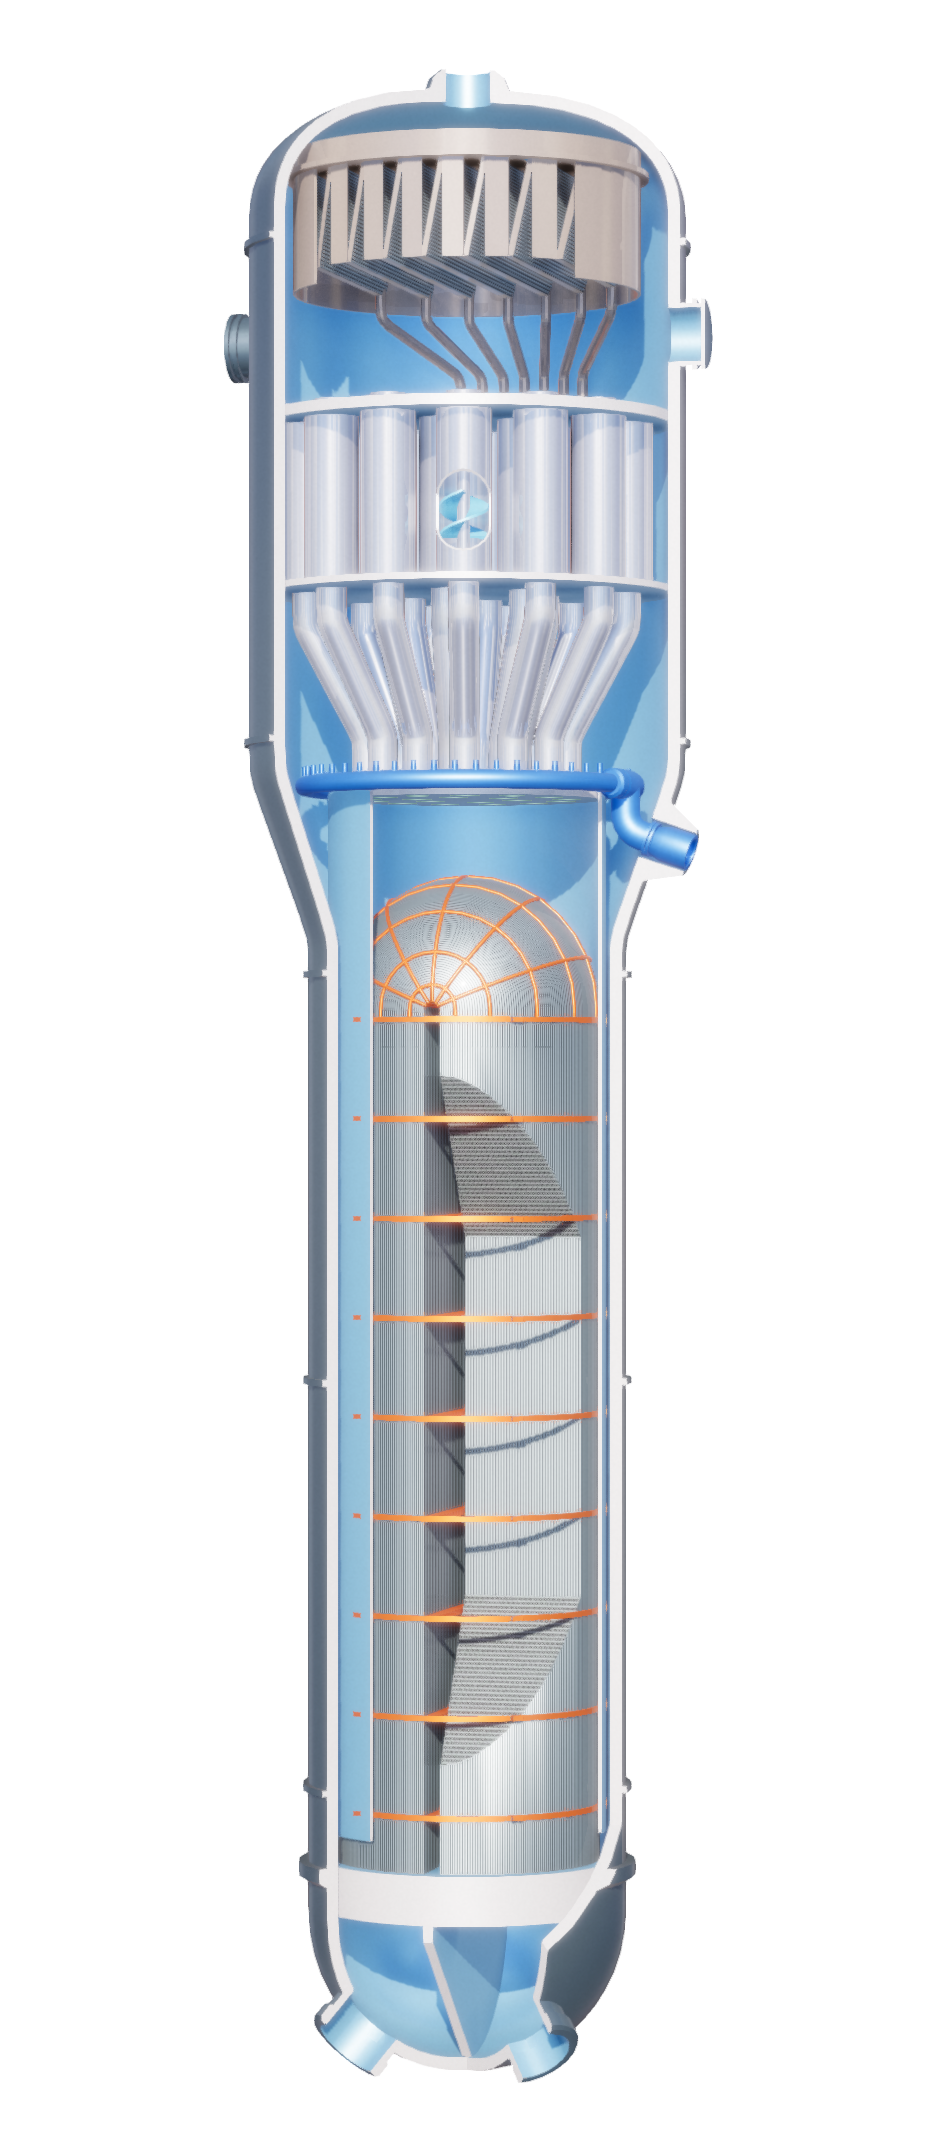
\includegraphics[width=\textwidth]{imgs/SG_PWR.png}
        \\[4pt]
        \footnotesize (a) \gls{pwr} steam generator
    \end{minipage}
    \hfill
    \begin{minipage}[b]{0.48\textwidth}
        \centering
        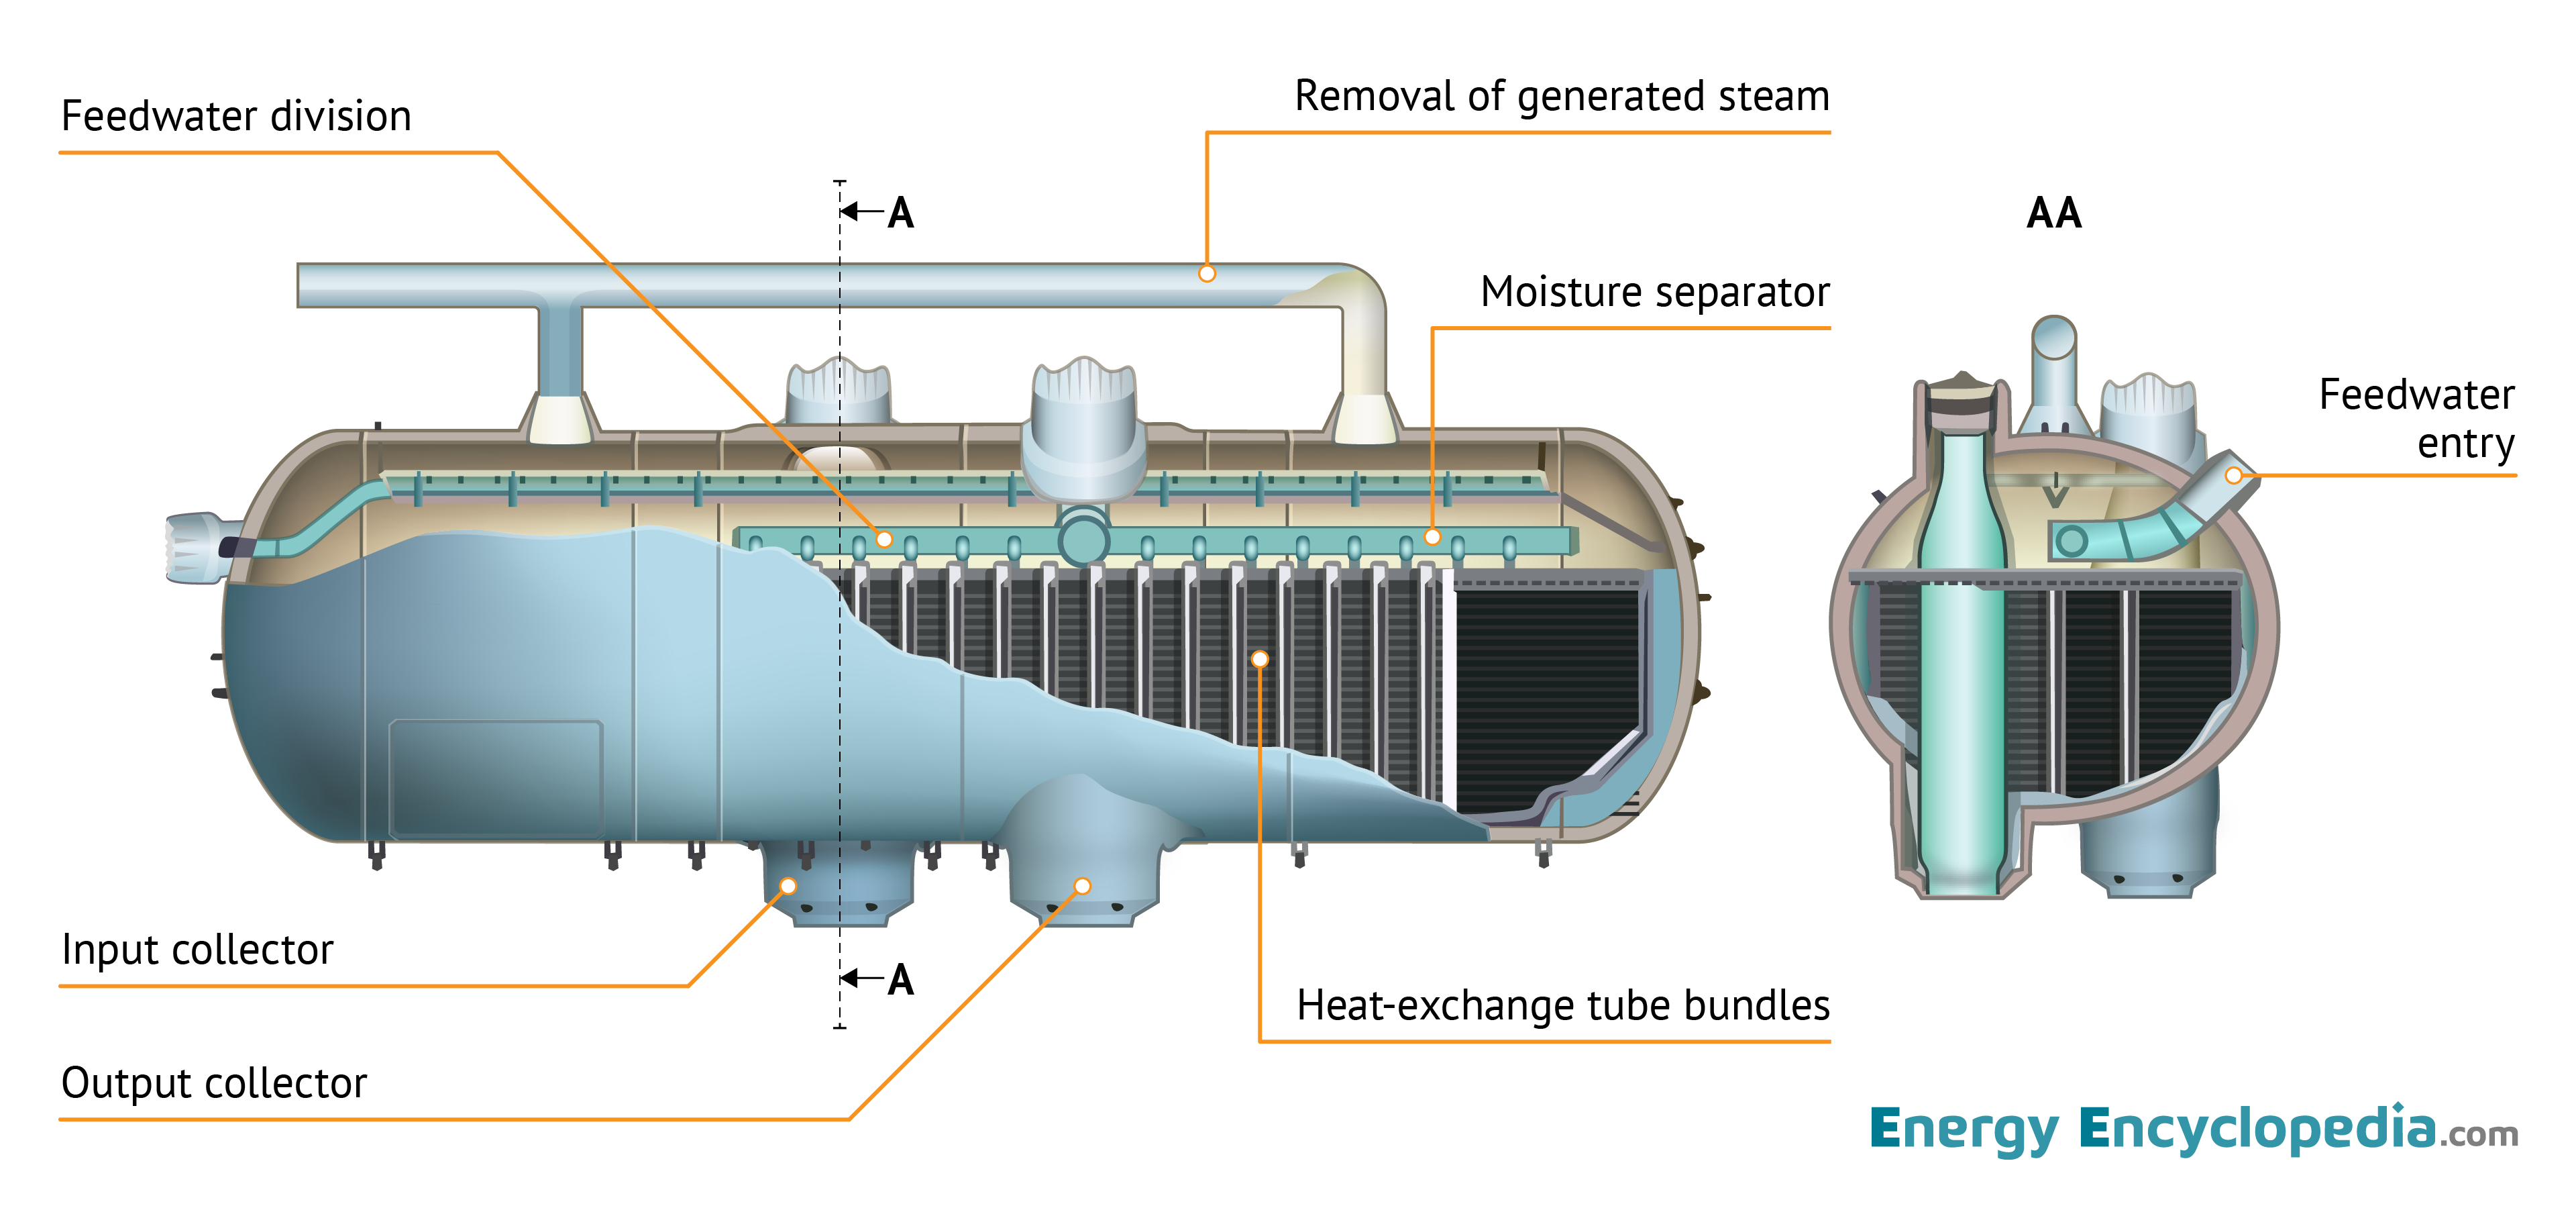
\includegraphics[width=\textwidth]{imgs/SG_VVER.png}
        \\[4pt]
        \footnotesize (b) \gls{vver} steam generator
    \end{minipage}
    \caption{Comparison of steam generator orientations in PWR (right, vertical) and VVER (left, horizontal) designs. Credit: energyencyclopedia.com}
    \label{fig:sg_orientations}
\end{figure}

Technological diversification occured also on other fronts as each nation developed its own reactor designs. The United Kingdom advanced gas-cooled Magnox reactors, the Soviet Union initiated development of the graphite-moderated, water-cooled RBMK design, while Canada's nuclear program focused on pressurized heavy water reactor (PHWR) technology, culminating in the first commercial CANDU reactor at Douglas Point in 1968 \cite{IAEA_PRIS_2025}.


\subsection{Generation II}
Between the 60s and 70s Generation II reactors were deployed, taking advantage of previous experience, reactors are now developed as commercial products rather then experiments or prototypes. In these decades numerous countries commissioned their first nuclear reactors: Belgium (1962), Italy (1963), Japan (1963), Sweden (1964), Switzerland (1969), Slovakia (1972), Argentina (1974), Bulgaria (1974) and Armenia (1976) \cite{IAEA_PRIS_2025}. Following the 1973 oil crisis, the deployment of nuclear power plants was accelerated in some countries as an energy security strategy. Most notably France implemented the Messmer Plan, named after the Prime Minister at the time, to greatly expand the nuclear plant fleet \cite{FundingUniverse_EDF_History_2025}. 

\begin{figure}[htbp]
    \centering
    
\includegraphics[width=0.7\textwidth]{imgs/placeholder.png}
    \caption{Map of first reactor deployments.}
    \label{fig:map_delopyments_npp}
\end{figure}

Nuclear expansion continued through the 1980s until 1986. As news from the Chernobyl disaster came to western countries, fear of the potential risks of nuclear power intensified. The public opposition grew significantly so that, even if safety and regulatory updates were implemented, several countries decided to slow down, reduce or halt their nuclear programs althogether, such was the case of Italy after the results of the 1987 referendum, which resulted in a complete phase-out of nuclear power \cite{MinisteroInterno_Referendum_1987, IAEA_PRIS_2025}. 

By the 1990s, multiple western countries had suspended nuclear deployment entirely, including Germany and Switzerland. France, previously the most active builder, connected 10 reactors between 1990-1999, while the United States and United Kingdom only deployed 4 and 1 reactors respectively during the same period. Italy completed its nuclear phase-out by 1990 with the permanent shutdown of all operating reactors \cite{IAEA_PRIS_2025}. 

Contrastingly, Eastern nations pursued an opposite trajectory. Following the post-Soviet economic transition, Russia resumed its nuclear program and has since continued expansion of its reactor fleet \cite{IAEA_PRIS_2025}. China initiated its nuclear program in the 1990s with Qinshan-1 (connected in 1991) and has since maintained aggressive expansion. Over the past three decades, China has brought 56 additional reactors online and currently has 29 under construction, positioning itself to surpass both France and the United States in total reactor capacity within the coming decade \cite{IAEA_PRIS_2025}.

\begin{figure}[htbp]
    \centering
    
\includegraphics[width=0.7\textwidth]{imgs/placeholder.png}
    \caption{Nuclear reactors deployment, per country throughout the years, with projections}
    \label{fig:npp_deployment_over_time}
\end{figure}

\subsection{Generation III}
As a result of the regulatory safety improvements, a stabilized choice of technology with LWRs settling as the to go choice all over the world and even larger capacities, Generation III reactor started to be developed in the 90s.

The improvement of these designs was fueled in the early 2000s by concerns over climate change, energy security, and rising fossil fuel prices, leading to Generation III+ reactors, such as the European Pressurized Reactor (EPR) or the US AP-1000 which improve safety and reliability in a consolidated plant layout. However after the 2011 Fukushima Daiichi accident, Western nations experienced a second setback: Germany accelerated its nuclear phase-out policy, while Italy reaffirmed its anti-nuclear position through another popular referendum \cite{MinisteroInterno_Referendum_2011}. In the following years projects faced substantial delays, cost overruns, and public opposition, with France's Flamanville-3 EPR serving as a particularly illustrative case experiencing budget increases to more then four times original estimates and construction timelines tripled from initial projections \cite{nea2020unlocking}.

\subsection{Generation IV}
From the late 2000s to nowadays, new nuclear commissioning projects such as Flamanville-3 can be classified as "Mega Projects", such term is used to refer to very large committments where economies of scale tend to fail due to the complexity of the task at hand, resulting in massive delays and cost overruns, well known examples of Mega Projects are Suez and Panama Canals, the Sydeny Opera House or the development of the Concorde Supersonic Aeroplane \cite{Flyvbjerg2014, BROOKES201557}. 

To counter this phenomena, the nuclear industry is developing Small Modular Reactors (SMRs) which are part of Generation IV reactors. SMRs are smaller, standardized reactors that can be built mostly off site to take advantage of economies of multiples. Some SMR designs are based on novelty technologies while others take advantage of well known water-based designs. 

Other generation IV reactors are being design to tackle on other aspects of nuclear power such as waste minimization or higher efficiencies. Manly by emplying different means of cooling to exploit neutrons at higher energies (fast neutrons), or by using thorium instead of uranium as fuel or even using direct gas based cycles to increase thermal efficiency.


\begin{figure}[htbp]
    \centering
    \begin{minipage}[b]{0.3\textwidth}
        \centering
        
\includegraphics[width=\textwidth]{imgs/placeholder.png}
        \\[4pt]
        \footnotesize (a) Gen IV example 1
    \end{minipage}
    \hfill
    \begin{minipage}[b]{0.3\textwidth}
        \centering
        
\includegraphics[width=\textwidth]{imgs/placeholder.png}
        \\[4pt]
        \footnotesize (b) Gen IV example 1
    \end{minipage}
        \hfill
    \begin{minipage}[b]{0.3\textwidth}
        \centering
        
\includegraphics[width=\textwidth]{imgs/placeholder.png}
        \\[4pt]
        \footnotesize (c) Gen IV example 1
    \end{minipage}
    \caption{Comparison of some gen IV designs}
    \label{fig:gen_IV_examples}
\end{figure}

\subsection{Current European Landscape}
In 2020, the COVID-19 pandemic exposed vulnerabilities in global economic systems and Russia's invasion of Ukraine in 2022 further revealed Europe's energy dependencies \cite{BRODNY2023121443, Sterling_European_Energy_Import_2025, EPRS_Energy_2023}. At the same time, decarbonization goals to combat climate change have prompted Western nations to reconsider nuclear energy as a valid power source able to provide low-carbon, reliable power while enhancing energy independence and system resilience \cite{EU2050ClimateStrategy}.

This strategic reassessment of nuclear is evident in recent policy initiatives. The European Union's classification of nuclear power as a sustainable investment under its taxonomy for climate mitigation \cite{EUTaxonomy}, alongside programs like the European Industrial Alliance on \glspl{smr} are a clear indicator of the renewed interest in nuclear technologies.

\textcolor{red}{I might add more...}

\section{Decision Support}
The historical overview demonstrates that nuclear energy decisions extend far beyond technical and economic considerations, inevitably encompassing social and political dimensions. This inherent complexity requires \glspl{dm} to evaluate numerous trade-offs across competing objectives in pursuit of balanced, optimal solutions. The systematic process of navigating trade-offs to arrive at informed choices constitutes the fundamental challenge of decision-making.

The decision making process begins by identifying the decision problem and the possible solutions to such problem. From this point, there are several ways to take the decision. The most common approach to decision making, which is encountered by anyone in our day to day life, is to look at the possible solutions or "alternatives", compare positive and negative outcomes based on own preferences and find the best, or less worst, between them.

For more complex situations such as those regarding energy systems, analytical frameworks, usually referred to as \gls{dss}, have been developed to support \glspl{dm}. In the realm of business and management \glspl{dss} are widely employed as softwares that collect and organize data, communications or knowledge to provide support by data analyses or visualization or by applying models. \cite{Power2023}.

The present study is focused on nuclear energy related decisions. The literature review will reveal that \gls{mcda} methods predominate in energy decision support research. This observation aligns with findings from Seran et al. (2025), whose comprehensive analysis of renewable energy studies demonstrated that the vast majority employed \gls{mcda} methodologies \cite{SERAN2025100044}.

\gls{mcda} systematically evaluates alternative solutions by decomposing decision problems into distinct criteria representing either the consequences of each alternative or their distinguishing characteristics \cite{ROY1990324}. This criterion-based approach offers two primary advantages: first, it enables the structured analysis of complex problems involving many criteria; second, it reveals preference patterns from different perspectives, which becomes particularly valuable when multiple stakeholders are involved. The method's transparency allows decision-makers to identify the most critical aspects of each alternative in relation to specific stakeholder preferences.

While there exists many \gls{mcda} methodologies (see Greco et Al. 2016 \cite{Köksalan2016} and Cinelli et al. 2020 \cite{CINELLI2020102261}) their common ground is to model the decision problem considering all availble information on it, considering trade-offs and then allowing to choose between alternatives \cite{HAAG2022105361}. \gls{mcda} can be used for solving different decision problems:
\begin{itemize}
\item Choice: Selecting the most preferred alternative(s) from a large pool of options.
\item Sorting: Classifying alternatives into predefined categories.
\item Ranking: Ordering all alternatives from most to least preferred.
\item Scoring: Ranking alternatives while also quantifying the differences between them.
\end{itemize}

A fundamental distinction exists between American and European \gls{mcda} methodologies. American-developed approaches, including the \gls{ahp} and \gls{mavt}, were born on the basis of the compensatory principle, emphasizing trade-off dynamics where a loss in one criterion can be offset by a gain in another.

In contrast, European researchers developed non-compensatory methods based on the outranking principle, such as ELECTRE and PROMETHEE. These methods establish preferences through binary outranking relationships between alternatives (e.g., "alternative A1 is preferred to A2 on regard to criterion C1") and may incorporate veto conditions between criteria. Unlike compensatory approaches, outranking methods were focused on meeting requirements rather than optimizing trade-offs \cite{HUANG2026103438, Köksalan2016}.

\section{Relevant Studies}
A review of relevant literature reveals numerous applications of MCDA methods across diverse fields. Focusing specifically on studies combining MCDA with nuclear power decision-making, several distinct approaches emerge:

Site selection studies represent the most common application, typically employing GIS-based software to evaluate potential locations for new nuclear installations within limited geographical regions. These analyses frequently incorporate quantitative non-technical factors such as population proximity \cite{DAMOOM2019110} \cite{BASEGMEZ2025105897}. Abdullah et al. (2025) extend this approach by including social dimensions like public acceptance and tourism impacts, which present challenges for quantification \cite{ABDULLAH2025105626}. Notably, Devanand et al. (2019) develop an algebraic optimization model to identify optimal SMR locations in Singapore, though like most site-focused studies, they favor a design without sistematic comparison \cite{DEVANAND2019339}.

A second category compares different nuclear technologies. Kiser and Otero (2023) evaluates PWRs, SMRs, and Molten Salt Reactors \cite{KISER2023104647}, while Locatelli and Mancini (2011) compares large and small reactor designs \cite{Locatelli01092012}. Birikorang's study stands out for its regional focus on South Africa and comparison of three specific reactor models (NuScale SMR, EM2-HTGR, FTR-MSR), though its technological comparisons mix designs at different maturity levels \cite{BIRIKORANG2026111837}. Notably, all three studies utilize the Analytic Hierarchy Process (AHP) or its Fuzzy variant. The last one (Birikorang) draws on the IAEA's INPRO methodology for advanced nuclear technology comparison \cite{IAEA_INPRO_2019}.

Broader energy comparison studies by Hernández-Torres (2025), Pasaoglu (2018), and Atilgan (2016) evaluate multiple generation options (typically eight alternatives) employing AHP-TOPSIS, AHP, and MAVT methodologies respectively. These studies use generic, averaged parameters for each technology class \cite{HERNANDEZTORRES2025122481,PASAOGLU2018654,ATILGAN2016168}. In contrast, Castelazo (2014) adopts a more precise approach using Multi-Attribute Value Theory (MAVT) to compare thirteen energy technologies, employing specific reference plants (e.g. EPR reactor for nuclear power) rather than generalized technology averages \cite{SANTOYOCASTELAZO2014119}.

Three studies show particular relevance to the current research. Zolkaffly et al. (2014) evaluates nuclear plant models in Malaysia but suffers from outdated data and neglects non-technical aspects \cite{10.1063/1.4866099}. Topaloğlu (2025) applies the Analytic Network Process (ANP) to compare reactor types (PWR, BWR, PHWR) and locations, though social considerations remain limited to site-specific factors \cite{TOPALOGLU2025103228}. Goushis (2025) employs TOPSIS to assess SMR deployment in the EU for coal replacement, but focuses on a single reactor model rather than comparative technology evaluation \cite{GOUSHIS2025126565}.

The literature review reveals four gaps in nuclear energy decision-making research. First, most studies focus solely on site selection rather than comparing different nuclear technologies. Second, comparisons between nuclear designs lack consideration of a specific decision-making context. Third, studies that do consider specific decision-making context, examine various energy generation options as broad technology categories (e.g., nuclear, solar, wind) rather than conducting detailed analyses of specific power plant designs. Fourth, social dimensions are frequently overlooked or applied only to site selection criteria.

\section{Observation on the validity of public surveys}
During this study's execution, multiple public surveys were reviewed based on the initial assumption that such instruments could provide quantitative measurements of qualitative factors such as public support for nuclear installations. However, the analysis exposed frequent methodological limitations introducing bias into the results. In Italy, a 2024 IPSOS survey commissioned by Legambiente (an environmental NGO with a known anti-nuclear position) reported 81\% opposition to nuclear power \cite{IPSOS_Nuclear_Survey_2024}. However, analysis of the survey report reveals problematic question design. The primary question was phrased as: \textit{"The debate on nuclear energy has returned to the forefront. What is your opinion on the matter?"} with response options structured as:
\begin{itemize}
    \item A1: "The current situation is complex; a return to nuclear should be evaluated"
    \item A2: "Nuclear has more risks than benefits and is not the right path"
    \item A3: "Nuclear energy entails excessive hidden costs and is not advantageous"
    \item A4: "Only safer technologies than current ones should be considered"
\end{itemize}

This framing demonstrates clear bias: two options (A2 and A3) explicitly oppose nuclear, A1 offers only conditional support, and A4 introduces safety concerns before suggesting potential support. Notably, the 81\% opposition figure includes A4 responses, which represent conditional rather than absolute opposition. When considering only explicit opposition (A2+A3), the figure decreases to 43\%.\\

A 2024 SWG study presents a more methodologically sound approach, though its conference presentation emphasized positive findings. The actual data reveals a more nuanced picture: over 80\% of respondents consider themselves insufficiently informed about nuclear topics, and further investigation found that approximately 90\% were unaware of SMRs or Generation IV reactors \cite{SWG_Nuclear_Survey_2024}. These findings suggest that public opinion on nuclear energy may be more influenced by lack of information than by firmly held positions.

\chapter{Methodology} % Pre processing

As presented in the literature review (Section \ref{sec:decision_support}), multiple \gls{mcda} methodologies exist, requiring an initial choice between outranking and value-based approaches. Outranking methods were discarded for this analysis, as no clear non-compensatory dynamics were evident in the decision context. Among American school methods, \gls{mavt} emerged as particularly suitable thanks to its value functions which offer significant advantages for capturing potential non-linearity in indicator values across their data ranges, a characteristic expected for economic and social criteria. While this method was previously introduced in the literature review (Section \ref{sec:decision_support}), the following paragraphs provide a detailed explaination.

\section{Applying MAVT to choose a Reactor}

\acrlong{mavt}, first presented by Keeney in 1996, is value-focused approach to decision-making that centers its analytical process on the core values and objectives of the \gls{dm}  rather than on the available alternatives. At the core of \gls{mavt} is the identification and quantification of what matters the most in a given decision context. This allows \glspl{dm} to explicitly define their \textit{fundamental objectives} (what they seek to achieve) rather then \textit{means objectives} (how those objectives will be achived). Preferences are modeled across performance ranges by means of value functions which are able to capture both linear and non-linear importance relationships between criterion values. Once the values of each criterion is established, criteriaare aggregated based on weights that convey the relative importance among criteria. The explicit nature of both value functions and weighting process make \gls{mavt} a particularly transparent decision analysis method, which is expecially valuable for research applications \cite{KEENEY1996537}.

The first methodological step requires \textbf{establishing indicators and their hierarchical structure}. Morton and Fasolo (2009) identify two traditional approaches: top-down and bottom-up \cite{Morton01022009}. The top-down approach begins with macro-level objectives that are subsequently decomposed into lower-level objectives through the guiding question "How can we achieve this?". On the other hand, the bottom-up approach, which is employed in the present study, starts with low-level objectives derived by comparing alternatives, asking: "What differentiates these alternatives?". Higher-level objectives are then constructed by aggregating similar indicators.

Morton and Fasolo note that top-down structuring tends to produce general value trees, difficult to apply to a specific study. Bottom-up approaches instead, create context-specific trees that are difficult to generalize. Additionally, this study found the bottom-up approach particularly useful in ensuring even indicator distribution across high-level objectives. This practice mitigates splitting bias, in which an objective divided into multiple sub-objectives will typically receive an higher cumulative weight than the equivalent single objective \cite{MARTTUNEN2018178}, accordingly, even distribution should prevent artificial favoring of objectives with greater indicator counts.


\textbf{Value Functions} are the characteristic feature of \gls{mavt} that allow to, first of all, reduce any metric, based on qualitative or quantitative data, to a scalar comparable with other different metrics. And second, it allows to convey more implicit information that a single metric can be able to carry. For example to evaluate a job offer, an obvius metric is its salary, in monetary terms. The perceived value, that is how the personal judgment of the salary, will never simply scale lineary with the amount of money recived, anything below a certain threshold dictated by monthly costs (e.g. rent, food, transportation etc) will have a significantly lower value then any offer above it. At the same time a hundred euro difference between two low salary offers might be considered much more significant then the same difference between two high offers. All this information can be conveyed with a specificcly tailored value function like the one shown in figure \ref{fig:value_function_example}.

\begin{figure}[H]
    \centering
    
\includegraphics[width=0.8\textwidth]{./imgs/placeholder.png}
    \caption{Example of a value function illustrating non-linear preferences.}
    \label{fig:value_function_example}
\end{figure}

\textcolor{red}{ricordati di dire che allinizio del capitolo abbiamo detto che a primo impato non cera evidence di non compensatory dynamic ma che poi vogliamo verificare questa cosa variando il metodo di aggregazione}

\textbf{Aggregation} within a fully compensatory framework, is typically performed using weighted summation (Equation \ref{eq:linear_aggregation}). The need to explore non-fully compensatory scenarios led to the development of alternative approaches employing nonlinear aggregation techniques (for a comprehensive description of aggregation methods see \cite{beliakov2007aggregation}). For the \gls{mcda} application of the present study the work by Langhans et al. (2014) \cite{LANGHANS2014494} and its implementation in the \gls{mcda} calculator tool \cite{PLACEHOLDER} will be followed, which includes the following aggregation methods:
\begin{itemize}
    \item Fully compensatory: \gls{sum} (equation \ref{eq:linear_aggregation})
    \item Partially compensatory: \gls{geo} (equation \ref{eq:geo_aggregation}) and \gls{har} (equation \ref{eq:har_aggregation})
    \item Non-compensatory: \gls{min} (equation \ref{eq:min_aggregation}) and \gls{max} (equation \ref{eq:max_aggregation})
\end{itemize}


\begin{equation}
   V_{sum} = \sum_{i=1}^{n} w_i \cdot v_i
   \label{eq:linear_aggregation}
\end{equation}


\begin{equation}
   V_{geo} = \prod_{i=1}^{n} v_i^{w_i}
   \label{eq:geo_aggregation}
\end{equation}

\begin{equation}
   V_{har} =
   \begin{cases}
   \frac{1}{\sum_{i=1}^{n} \frac{w_i}{v_i}} & \text{if } v_i > 0 \text{ for all } i, \\
   0 & \text{otherwise}
   \end{cases}
   \label{eq:har_aggregation}
\end{equation}

\begin{equation}
   V_{min} = \min_{i=1,\dots,n} v_i
   \label{eq:min_aggregation}
\end{equation}

\begin{equation}
   V_{max} = \max_{i=1,\dots,n} v_i
   \label{eq:max_aggregation}
\end{equation}

Equations \ref{eq:linear_aggregation}, \ref{eq:geo_aggregation} and \ref{eq:har_aggregation} are subject to the normalization condition $\sum_{i=1}^{n} w_i = 1$

\textbf{Elicitation of weights} in \gls{mcda} varies according to methodological choices. While survey-based approaches using direct elicitation methods (e.g., ranking criteria or expressing judgments) offer simplicity and intuitiveness for general public participation, they face significant criticism from experts. Morton and Fasolo (2009) \cite{Morton01022009} highlight fundamental concerns: "People's ability to understand and respond to direct importance questions baffles us. Both of us regard such questions as meaningless and refuse to answer them. It could be that our intuitions have been destroyed by our atypically extensive exposure to DA." Reichert et al. (2015) \cite{REICHERT2015316} recommend a differentiated approach: technical criteria should be weighted through expert elicitation, while higher-level objectives reflecting major societal trade-offs may incorporate population or stakeholder opinions.

More sophisticated methods like swing elicitation \cite{Goodwin_Wright_2004}, present challenges for public comprehension. Aubert et al. (2020) \cite{AUBERT2020100156} demonstrated this limitation when approximately 73\% of general public respondents failed to correctly understand the swing elicitation method in their study (later utilized by Haag et al., 2022 \cite{HAAG2022105361}) \footnote{Swing elicitation is an indirect weighting method that evaluates the relative importance of improvements between worst and best-case scenarios for different criteria. For example: \textit{"On a scale from 1 to 10, how much more important is increasing your salary from €1,200 (minimum wage) to €1,800 (market maximum) compared to increasing annual paid leave from 4 weeks (legal minimum) to 12 weeks (market maximum)?"}}.

Rezaei (2015) proposed the \gls{bwm} which first identifies the most and least important criteria and then performs pairwise comparisons between these two reference criteria and all others \cite{REZAEI201549}. This method reduces the number of evaluation required: given $n$ criteria to evaluate, only $2n-3$ pairwise comparisons are needed, against the $\frac{n(n-1)}{2}$ available unique pairs. Another significant advantage is that this method allows for consistency checks to verify the results of the elicitation process.

Liang et al. (2022) proposed the \gls{bwt} which combines the range sensitivity of methods like swing elicitation with the possibility to perform consistency checks offered by \gls{bwm} \cite{LIANG2022957}.

\textcolor{red}{[Detailed BWM explanation to be added]}



\chapter{Case Study} % Main analysis
\label{sec:case_study}
\section{Definition of the Study Context}
\subsection{Country Selection for Comparative Analysis}
This study evaluates four European countries: France, Italy, Poland, and Switzerland, to assess how national energy contexts influence the ranking of nuclear reactor designs \footnote{Data regarding electricity loads and cross border flows is source from the ENTSO-E Transparency Platform and refers to data from 2024 \cite{ENTSOE_Transparency_2025}. Data analysis can be found at \textcolor{red}{ADD LINK !!!!!!!!}}.
--- try to justify why Europe and why select some... Still, there is no enough rationale for selecting these four countries---

\textbf{Italy}'s nuclear landscape is constrained by the 1987 post-Chernobyl referendum which mandated complete phase-out of nuclear power and its 2011 reaffirmation following Fukushima. However, since Italian referendums are abrogative rather than prescriptive, government decrees are enough to reverse these policies \cite{Costituzione_Italiana_Art75_1947}. The current administration seems willing to reintroduce nuclear power \cite{Sole24Ore_Italy_Nuclear_Strategy_2024}, however, Italy's history of political volatility and the long-term nature of nuclear projects create significant implementation challenges regardless of public opinion trends. 

For this study we have taken into consideration only the northern part of Italy due to the country's fragmented electricity market structure. The north bidding zone is the most energy-intensive with an average load of 17.66 $\pm$ 4.35 GW, for reference, by analysing data from the Italian \gls{tso} \cite{Terna_Italian_Electricity_Demand_2024} and the Italian institute for statistics \cite{ISTAT_POS_2024}, it is possible to conclude that the North bidding zone, despite only hosting 35\% of the Italian population, represents 56\% of the total electric demand. In addition to the significant load, the bidding zone has a substantial dependence on imports, which averaged 5.23 $\pm$ 1.67 GW in 2024, accounting for almost 30\% of its electric demand. Analysis of cross-border flow data shows that imports are active 99\% hours of the year. 

\paragraph{Poland} shows strong public backing for nuclear energy development, with surveys reporting up to $92\%$ support \cite{NucNet_Poland_Nuclear_Support_2024}. The public sentiment aligns with tangible progress in the country's nuclear program, including preliminary site works and vendor agreements \cite{Westinghouse_Poland_Nuclear_2025,WorldNuclearNews_Poland_Preliminary_Works_2025}, suggesting robust governmental commitment to nuclear deployment. The Polish grid produced 55\% of its electricity with coal \cite{IEA_Electricity_2024}, making it the country with the highest green house gas emission intensity in Europe \cite{ElectricityMaps_CarbonIntensity_2024}.


\paragraph{Switzerland} presents a more complex picture. Following the 2011 Fukushima accident, the government adopted a phase-out policy later confirmed by a referendum in 2017 \cite{WorldNuclear_Switzerland_Profile_2025}. However, recent surveys indicate shifting public opinion, with $53\%$ now supporting nuclear power \cite{Euronuclear_Swiss_Nuclear_Poll_2023,NucNet_Nuclear_Support_Survey_2023,WorldNuclearNews_Swiss_Nuclear_Poll_2023}. The federal government has subsequently signalled potential reconsideration of nuclear role in meeting climate targets \cite{swissinfo_Nuclear_Power_Switzerland_2025}, though the narrow margin of support and Switzerland's direct democracy system create policy uncertainty. 

The Swiss grid is characterized by a low demand, averaging 6.79 $\pm$ 1.12 GW, and generation dominated by renewables (65\% average share) particularly hydroelectric which provided 59\% of the electricity in 2024 \cite{IEA_Electricity_2024}. This high dependence on renewables is reflected on substantial cross border flow variability which average 2.71 $\pm$ 3.14 GW. The large standard deviation reflects the oscillating nature of the Swiss cross-border flows, consequence of periodic exports due to overproduction, alternating with imports when renewable output is low.\\

\paragraph{France} demonstrates consistent public support for nuclear energy, with 75\% favouring continued operation of existing plants and $65\%$ supporting new construction according to a 2022 survey \cite{IFOP_Nuclear_Perception_2023}. Given the long-standing consensus on nuclear power as a strategic energy pillar and the country's established industrial base, significant policy reversals appear unlikely. The country electric grid relies heavily on nuclear power, which accounted for 67\% of its electricity generation \cite{IEA_Electricity_2024}. Despite the substantial demand, which averaged $49.05 \pm 9.83$ GW, France is a net electricity exporter, with 21\% of total domestic production crossing the border to neighbouring countries.

\subsection{Selection of Reactor Models}
This study focuses on a curated set of reactor designs at an advanced stage of development.
The selection process begins with the analysis of the \gls{iaea} "Nuclear Reactors in the World" publication \cite{international2024iaea}, which catalogues operational, under-construction, and decommissioned reactors globally. \\

The initial selection process applied two primary exclusion criteria. First, designs were eliminated based on supplier origin, removing all reactors associated with countries unlikely to engage in nuclear technology transfer with European countries, namely, Russia, China and India. Second, reactors commissioned before 2000 were excluded from consideration, as their designs represent outdated technological standards \footnote{The complete filtering is documented in the accompanying analysis notebook \textcolor{red}{ADD LINK !!!!!!!!}}.

From this pre-selected group, three designs were prioritized for comprehensive analysis: the \gls{epr}-1750, \gls{apr}, and \gls{ap}. It should be noted that while the \gls{epr} (1650 MWe) and \gls{epr}-1750 share significant design similarities, they are treated as separate models in this study. Additionally, the \gls{abwr}, though listed as operational in the \gls{iaea} \gls{aris} database, was excluded following verification through the \gls{pris} database, which indicates that all \gls{abwr} units have suspended operation since 2011 \cite{IAEA_PRIS_2025}. The selection process and its outcomes are summarized in Table \ref{tab:reactor-selection}.

The author acknowledges the controversy between Westinghouse and KEPCO regarding the APR design derivation from the System 80 design. However, as no official documentation prohibits its commercialization in Europe, and considering recent evaluations of the Korean design (including the 2023 Czech tender, though later contested by \gls{edf} and Westinghouse \cite{WNN_Czech_Nuclear_Appeal_2024}), the \gls{apr} has been included in this analysis.

The \gls{epr}2 and \gls{epr}1200 designs, while reviewed positively by the French nuclear safety authority \cite{WNN_EPR1200_Safety_2023}, lack commercial commitments (the gls{epr}1200 was proposed for the Czech tender but ultimately unsuccessful \cite{WNN_Czech_Nuclear_Appeal_2024}). Moreover, considering their absence from the ARIS database and overall limited available technical documentation, these \gls{edf} designs have been excluded from the current study.


\begin{table}[!hb]
\centering
\begin{tabularx}{\textwidth}{llXXXX}
\toprule
\textbf{Reactor Name} & \textbf{Country} & \textbf{Technology-sharing} & \textbf{Commercial Operation} & \textbf{Up to Date} & \textbf{Decision} \\
\midrule
\gls{apr} & S.Korea & \cmark & \cmark & \cmark & \textbf{Selected} \\

CAREM Prototyp & Argentina & \cmark & \xmark & \cmark & Rejected \\

PRE KONVOI & Germany & \cmark & \cmark & \xmark & Rejected \\

\gls{epr} 1750 & France & \cmark & \cmark & \cmark & \textbf{Selected} \\

\gls{ap} & USA & \cmark & \cmark & \cmark & \textbf{Selected} \\

\gls{abwr} & Japan & \cmark & \xmark & \cmark & Rejected \\

\gls{apwr} & Japan & \cmark & \xmark & \cmark & Rejected \\

\gls{epr} & France & \cmark & \cmark & \xmark & Rejected \\

OPR-1000 & S.Korea & \cmark & \cmark & \xmark & Rejected \\
\bottomrule
\end{tabularx}
\caption{Selection of reactor models for analysis}
\label{tab:reactor-selection}
\end{table}


Subsequently, the \gls{iaea} \gls{aris} database \cite{iaea2025aris}, was consulted to identify advanced reactor models classified as under design, under regulatory review, under construction, or operational. To avoid redundancy, Generation III+ designs captured in both \gls{aris} and \gls{pris} datasets were removed. Demonstrations units and prototypes were also excluded from this set, yielding 10 candidate designs. Each of them was then assessed for development status, technological readiness, and applicability to European deployment as summarized in Table \ref{tab:advanced-reactor-selection}.

\begin{table}[!hb]
\centering
\begin{tabularx}{\textwidth}{lllX}
\toprule
\textbf{Reactor Name} & \textbf{Country} & \textbf{Used} & \textbf{Reasoning} \\
\midrule

APR+ & S.Korea & \xmark & As reported in the manufacturer website \cite{kepcoenc2025} this design is mean to be an "indigenous reactor cleared of obstacles to export"\\

ATMEA & Japan, France & \xmark & Joint venture was abandoned in 2019 \cite{PLACEHOLDER}\\

BWRX300 & USA, Canada & \cmark & Design from GE-Hitachi, a lot of support from US and Canada as well as interes in the EU \cite{wnn2025bwrx300} \cite{wnn2025hungarysmr}.\\

i-SMR & S.Korea & \xmark & Never expressed interest in development outside south Asia and the middle east, no updates since early 2024.\\

iMSR400 & US & \xmark & No interest overseas, project seems to be at an early stage of development.\\

Natrium & US & \xmark & Demo plant \cite{terrapower2025natrium}.\\

Nuward & France & \xmark & After the change in direction of 2024 the project has been set back \cite{PLACEHOLDER}.\\

Nuscale & US & \cmark & Even if there was some financial controversy in 2024 \cite{PLACEHOLDER}. the project seems to be still moving forward in terms of goverment founding \cite{PLACEHOLDER} and regulatory review \cite{PLACEHOLDER}.\\

PRISM & US & \xmark & GE-Hitachi considers it a "concept ... currently being put into practice in two reactors: Natrium and ARC-100" \cite{PLACEHOLDER}.\\

Rolls Royce SMR & UK & \cmark & It's moving forward and from the technological point of view this is the simples as it it litteraly a scaled down PWR\cite{PLACEHOLDER}.\\

SMART & S.Korea, Saudi Arabia & \xmark & Plan to export only to south-east asia and middle east \cite{wnn2025smrdesign}.\\ \bottomrule

\end{tabularx}
\caption{Selection of advanced reactor models for analysis}
\label{tab:advanced-reactor-selection}
\end{table}

\subsection{Overview of the case study}
The overall selection produced a set of six reactors, three Generation III+ and three \glspl{smr}. Their main characteristics are summarized in Table \ref{tab:final-reactor-selection}. The most notable differences are the integrated designs of the \gls{bwrx} and Nuscale \gls{smr} which eliminate external primary loops in favour of steam generators positioned inside the reactor pressure vessel. This allows to reduce the overall size and to exploit natural circulation for cooling. The \gls{npm}, referred to as US460 in technical documentation, is the only model designed to be deployed in a multi unit configuration, with up to 12 modules in the same containment building, for this study the 6 module plant (VOYGR-6) has been selected as it recently revived the \gls{sda} by the US Nuclear Regulatory Commission in May 2025 \footnote{\textit{"A standard design approval indicates that a proposed reactor design meets applicable agency safety requirements. Companies that seek to use the US460 design would have to file applications seeking permission to build and operate a nuclear reactor using the approved design"} \cite{NRC_2025_033}}.

\begin{table}[!hb]
\centering
\begin{tabularx}{\textwidth}{lclcX}
\toprule
\textbf{Reactor Name} & \textbf{Type} & \textbf{Construction} & \textbf{P$_e$ (MWe)} & \textbf{Supplier} \\
\midrule
\gls{apr} & \gls{pwr}  & 1 Unit & 1340 & KEPCO (S.Korea) \\
\gls{epr} 1750 & \gls{pwr}  & 1 Unit & 1630 & Framatome (France) \\
\gls{ap} & \gls{pwr}  & 1 Unit & 1120 & Westinghouse (USA) \\
\gls{bwrx} & \gls{ibwr} & 1 Unit & 300 & GE-Hitachi (USA)\\
Rolls Royce SMR & \gls{pwr}  & 4 to 12 Units & 470 & Rolls Royce (UK) \\
Nuscale & \gls{ipwr} & 1 Unit & 77 & Nuscale Power (USA) \\
\bottomrule
\end{tabularx}
\caption{Final selection of reactor models for analysis}
\label{tab:final-reactor-selection}
\end{table}

 % Detailed Definition of the Case Study
\section{Step 2: Definition of the indicators}
\label{sec:brainstorming_indicators}
The initial phase of this \gls{mcda} study focuses on indicator selection and hierarchical structuring. The following sections outline the methodological process employed to develop the final indicator set. It should be noted that this study primarily evaluates the feasibility of the proposed approach rather than generating definitive results. Accordingly, this study serves to identify which indicators or areas may require further detailed development in future iterations, as the weighting process will naturally reveal priority areas. Indicators receiving minimal weights may not justify further refinement, while those with substantial weights could benefit from more granular analysis. With this context established, the subsequent sections present the process that resulted in the final indicator set used in this study.


Following the bottom-up approach outlined in Section \ref{sec:mavt_presentation}, the initial analytical step involved identifying all potential differentiating factors among the six reactor alternatives. The process began with a series of personal brainstorming sessions by the author, followed by a preliminary selection phase. The resulting comprehensive list of 35 potential indicators\footnote{The complete list is available as a CSV file in the repository, with an example Python script provided for navigation (see Section \ref{sec:appendix_code} for details)} was then extensively reviewed with the support of three domain experts to evaluate:
\begin{itemize}
    \item Completeness (identifying missing aspects)
    \item Redundancy (eliminating repetitive measures)
    \item Relevance (removing irrelevant indicators)
    \item Granularity (balancing overly specific or aggregate measures)
\end{itemize}

Further discussion with several experts from different backgrounds was helpful to identify other possible aspects, as well as to collect feedback that helped improve the justifications. On this regard it is really important that the analyst takes into serious consideration every suggestion provided by others, and, whenever these have to be discarded, it is important to report it and properly justify the omission to ensure full transparency.


As anticipated, the extensive indicator list required systematic screening for several reasons:
\begin{itemize}
    \item Double counting: The same aspects might be represented by multiple indicators, leading to biased weights
    \item Scope: Some aspects might be valid but not relevant for the point of view of the study, in this case, European governmental agencies
    \item Data availability: This wouldn't be the case for a field application but for the purpose of this thesis obtaining data outside the public domain was deemed unfeasible.
\end{itemize}

Table \ref{tab:screening-indicators} provides examples of excluded indicators. The most significant exclusions are justified in Section \ref{sec:indicators_removed} while possible improvements for future studies are documented in Section \ref{sec:results}.


\begin{table}[!hb]
\centering
\begin{tabularx}{0.8\textwidth}{Xccccc}
\toprule
\textbf{Indicator} & \textbf{F1} & \textbf{F2} & \textbf{F3} & \textbf{Decision} \\
\midrule
Load Following Capabilities & \cmark & \cmark & \cmark & \textbf{Selected} \\

Mining waste & \cmark & \cmark & \xmark & Rejected \\

Land Usage & \xmark & \xmark & \cmark & Rejected \\

Core Damage Frequency & \xmark & \cmark & \cmark & Rejected \\

Spent Nuclear Fuel & \cmark & \cmark & \cmark & \textbf{Selected} \\

Local Economy Turnaround & \xmark & \xmark & \cmark & Rejected \\

Capital Investment Budgeted & \cmark & \cmark & \cmark & \textbf{Selected} \\

Supplier Availability  & \cmark & \cmark & \cmark & \textbf{Selected} \\
\bottomrule
\end{tabularx}
\caption{Example of the selection process of indicators. F1: High relevance to the case study, F2: Data is available, F3: Not redundant nor highly correlated with other indicators}
\label{tab:screening-indicators}
\end{table}

Following this systematic screening process, twelve indicators remained and were subsequently aggregated into higher-level objectives, presented in Table \ref{tab:final_indicators}. In this bottom-up approach, each group collects indicators that share a common high-level point of view. The subsequent sections describe each retained indicator, covering its data sources, conceptual explanations, and the methodological rationale for its inclusion.

\begin{table}[!hb]
    \centering
    \begin{tabularx}{\textwidth}{lllX}
        \toprule
        \multicolumn{4}{c}{\textbf{Technical Indicators}} \\
        \midrule
        T1 & Thermal Efficiency & [\%] & Indicator of the thermal hydraulics efficiency \\
        \cmidrule(lr){1-4}
        T2 & Discharge Burnup & [GWd/tonHM] & Indicator of the fuel utilization efficiency and neutron economy \\
        \cmidrule(lr){1-4}
        T3 & Net Power Output & [MWe] & How much does the output of one unit fit the grid demand \\
        \cmidrule(lr){1-4}
        T4 & Load Following Capabilities & [-] & How much do the load following capabilities satisfy the grid demand \\
        \midrule
        \multicolumn{4}{c}{\textbf{Feasibility Indicators}} \\
        \midrule
        F1 & Design Maturity & [Score] & Technological readiness of the design \\
        \cmidrule(lr){1-4}
        F2 & Licensing Status & [Score] & How close to having a licence is the reactor? \\
        \cmidrule(lr){1-4}
        F3 & Supplier Availability & [Score] & Is the supplier established in the country? Even partially, for instance has offices \\
        \midrule
        \multicolumn{4}{c}{\textbf{Economic Indicators}} \\
        \midrule
        E1 & Capital Investment Budgeted & [2024EUR/kWe] & Overnight, budgeted construction costs (estimates include decommissioning etc.) \\
        \cmidrule(lr){1-4}
        E2 & Design Complexity & [Score] & From which delays in the manufacturing processes might arise \\
        \cmidrule(lr){1-4}
        E3 & Construction Complexity & [Score] & From which delays in the building processes might arise \\
        \cmidrule(lr){1-4}
        E4 & Operative and Fuel Costs & [USD2020/MWh] & Ongoing costs \\
        \midrule
        \multicolumn{4}{c}{\textbf{Social Indicators}} \\
        \midrule
        P1 & Electricity Market Benefit & [2024EUR/MWh] & Potential reduction of cost in the Electricity Market by marginal price logic, by constructing one unit \\
        \cmidrule(lr){1-4}
        P2 & GHGe Benefit & [tonCO2eq] & Potential Yearly Reduction on GHG Emissions by installing one unit \\
        \cmidrule(lr){1-4}
        P3 & Perceived Safety & [Score] & Based on public opinion, how much each reactor sounds safe? \\
        \cmidrule(lr){1-4}
        P4 & Nuclear Waste & [tonSNF] & Estimation of amount of spent fuel produced \\
        \bottomrule
    \end{tabularx}
    \caption{Final selection of indicators, categorized and coded for evaluation.}
    \label{tab:final_indicators}
\end{table}
 % Definition of the 
\subsection{Technical parameters}
The frist set of indicators are technical parameters that define the performance of each reactor design form an engineering standpoint.
An overview of technical parameters is presented in Table \ref{tab:indicators-technical}.

\textbf{Thermal efficiency} indicates the fraction of thermal power generated by fission that is converted into net electrical power, accounting for in-plant consumption. Efficiency values were calculated using net electrical power output and thermal power data from the \gls{aris} database \cite{iaea2025aris}:
$$
\eta = \frac{P_{el,net}}{P_{th}}
$$
This indicator is a way to judge the thermal-hydraulic design of the reactor.

\textbf{Discharge Burnup} measures the energy extracted per unit of heavy metal from the nuclear fuel ($MWd/tonHM$). Data for APR1400 and AP1000 were sourced from the \gls{aris} database \cite{iaea2025aris}, while EPR 1750 data were obtained from \cite{NRC_ML052280170}. Ranges are provided for SMRs due to design variability. Such value is indicative of the neutronics and core design of the reactor.


\textbf{Net Power Output} has to be considered when choosing a power plant in relation to the needs of the local energy market, for instance a country that is constantly importing a substantial amount of energy might prefer large power plants rather then \glspl{smr}, on the other hand countries where renewable energy dominates the mix, small and flexible power could be preferred. For three large reactors data was sourced from \cite{IAEA_PRIS_2025} while for \glspl{smr} data was obtained from \cite{iaea2025aris}.


\textbf{\glspl{lfc}} can be quantitatively assessed using characteristic curves that represent ramp-up and ramp-down rates as a function of load (expressed as percentage of nominal power $\%P_{nom}$), as illustrated in Figure \ref{fig:load-following-curve}. To facilitate comparative analysis, these performance curves are reduced to scalar values through integration of the area under said curve.

\begin{figure}[!hb]
    \centering
    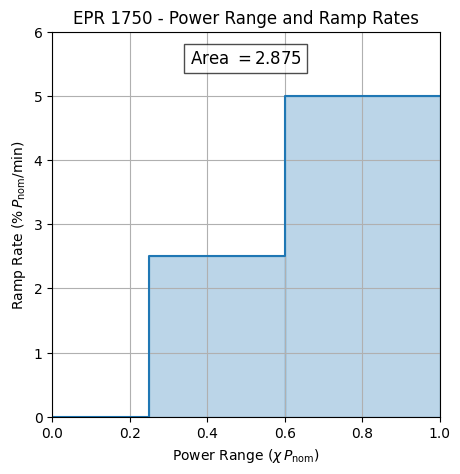
\includegraphics[width=0.7\textwidth]{imgs/load_following_curve.png}
    \caption{Example \gls{lfc} curve for EPR-1750}
    \label{fig:load-following-curve}
\end{figure}

For benchmarking purposes, the \gls{lfc} of a pair a tipical gas powered plant was computed. Specifically, a combined cyle plant featuring two heavy-duty \gls{ge} 9HA.02 gas turbines (2015 data) \cite{GE_9HA_Gas_Turbine_2015}. 
Sources for load following data for APR1400, AP1000, BWRX-300 and Rolls Royce SMR where sourced from \cite{iaea2025aris}, while EPR 1750 data was obtained from \cite{OECD_NEA_Load_Following_2011}. For NuScale data was sourced from \cite{ENCO_SMR_Analysis_2022}.

\begin{table}[!ht]
    \centering
    \begin{tabularx}{0.6\textwidth}{l X X}
        \toprule
        \textbf{Reactor Model} & \textbf{S1} & \textbf{S2}\\
        \midrule
        APR1400           & 1340 & 0.21 \\
        EPR 1750          & 1630 & 2.88 \\
        AP1000            & 1120 & 4.25 \\
        BWRX-300          & 300 & 0.25 \\
        Rolls Royce SMR   & 470 & 2.00 \\
        NuScale (Voygr-6) & 462  & 2.00 \\
        \gls{ge} 9HA.02 2xCC    & 1515 & 7.02 \\
        \bottomrule
    \end{tabularx}
    \caption{System Indicators: S1: Net Electric Power Output [$MW_{e,net}$], S2: \gls{lfc} [$\%P_{nom}/min$]}
    \label{tab:indicators-system}
\end{table} % Definition of Technical Indicators
\subsection{Feasibility Indicators}
This group reflects the concerns of any skeptical party that might argue about the feasibility of the commissioning process itself. These indicators capture all practical factors that may influence implementation ease, with evaluations conducted using qualitative scales based on current conditions (status quo) as detailed in the following analysis. All of the indicators in this group are qualitative in nature, the detailed methodology to charaterize them is presented in section \ref{sec:qi}. Hereafter, each indicator is described as well as the reason behind their starting point evaluation.

\paragraph{Design Maturity}
Design maturity was evaluated on an ordinal scale reflecting current deployment status. Among large reactors, the \gls{epr} received a 4/5 score due to its limited construction experience, while both \gls{apr} and \gls{ap} achieved 5/5 ratings. For \gls{smr} designs, only the Rolls-Royce reactor scored 2/5 rather than 1/5, as its design closely resembles existing \glspl{pwr} featuring forced circulation and external steam generators. Table \ref{tab:maturity-comparison} presents the supporting data for this preliminary maturity assessment.

\begin{table}[htbp]
    \centering
    \renewcommand{\tabularxcolumn}[1]{m{#1}}
    \begin{tabularx}{\textwidth}{Xcccccc}
        \toprule
        \textbf{Parameter} & \textbf{APR} & \textbf{EPR} & \textbf{AP} & \textbf{BWRX} & \textbf{Rolls Royce} & \textbf{NuScale} \\
        \midrule
        Operational units & 9 & 2 (+2) & 7 & 0 & 0 & 0 \\
        \cmidrule(lr){1-7}
        Under construction & 3 & 2 & 2 & 0 & 0 & 0 \\
        \cmidrule(lr){1-7}
        Technology & PWR & PWR & PWR & i-BWR & PWR & i-PWR \\
        \cmidrule(lr){1-7}
        Construction strategy (Units) & 1 & 1 & 1 & 1 & 1 & 4–12  \\
        \cmidrule(lr){1-7}
        Fuel & Existing & Existing & Existing & Existing & Variation & Variation \\
        \cmidrule(lr){1-7}
        Design Maturity Score & 5/5 & 4/5 & 5/5 & 1/5 & 2/5 & 1/5 \\
        \bottomrule
    \end{tabularx}
    \caption{Data to support design maturity.}
    \label{tab:maturity-comparison}
\end{table}


\paragraph{Licensing Status}
Licensing progress was evaluated based on each reactor current regulatory status within the European context. The three conventional reactors received baseline scores of 4/5 due to their established international licensing history, with the \gls{epr} achieving 5/5 given its existing European deployments, with the previous iteration, in France and Finland \footnote{For clarity regarding nuclear reactor nomenclature: Internet searches for "EPR" will present results for Flamanville and Olkiluoto plants as well as UK units (Hinkley Point and Sizewell) and China's Taishan plant. This is actually an aggregation of two distinct designs: the original 1600 MWe "European Pressurized Reactor" (Flamanville/Olkiluoto) and the evolved 1750 MWe "Evolutionary Pressurized Reactor" (Hinkley Point/Sizewell/Taishan) analyzed in this study.}.


For \glspl{smr} designs, NuScale and Rolls-Royce received 1/5 scores as their licensing processes remain confined to overseas markets (United States for NuScale; United States and United Kingdom for Rolls-Royce). The \gls{bwrx} was assigned 2/5 despite similar overseas licensing status (United States, United Kingdom, and Canada) to acknowledge three distinguishing factors: exceptional financing support (scoring 6/6 in the \gls{nea} \gls{smr} Dashboard \cite{NEA_SMR_Dashboard_2025}), the issue of a Canadian building permit, and utilization of existing fuel designs that eliminate requirements for new fuel licensing procedures. The 3/5 score was intentionally omitted to clearly differentiate between established and emerging reactor designs. Table \ref{tab:licensing_info} summarizes the licensing status evaluation.
\begin{table}[!hb]
    \begin{tabularx}{\textwidth}{l>{\centering\arraybackslash}X}
        \toprule
        \textbf{Reactor Model} & \textbf{Information} \\
        \midrule
        APR-1400 &
          \begin{itemize}
            \item Built in Korea, UAE
            \item Licensed in US
            \item Approved by EUR
          \end{itemize} \\
        \midrule
        EPR-1750 &
          \begin{itemize}
            \item Built in UK, China (+ FR, FIN)
            \item Approved by EUR
          \end{itemize} \\
        \midrule
        AP-1000 &
          \begin{itemize}
            \item Built in China, US
            \item Approved by EUR
          \end{itemize} \\
        \midrule
        BWRX-300 &
          \begin{itemize}
            \item Build license in CAN 2025 (subject to VDR 2023)
            \item Pre-application in US in 2019
            \item UK GDA started 2024
          \end{itemize} \\
        \midrule
        Rolls Royce SMR &
          \begin{itemize}
            \item Pre-application in US in 2025
            \item UK GDA started in 2022
          \end{itemize} \\
        \midrule
        NuScale &
          \begin{itemize}
            \item SDA in US (2025)
          \end{itemize} \\
        \bottomrule
    \end{tabularx}
    \caption{Licensing and construction information for selected reactor models.}
    \label{tab:licensing_info}
\end{table}

\paragraph{Supplier Availability}
Market entry ease and local industry involvement significantly affect commissioning timelines and national economic benefits, both of which are key considerations for governmental agencies. While a comprehensive evaluation would require detailed analysis of each country's nuclear industry status and expansion potential, this preliminary study implements a simplified assessment approach.

The methodology employs a country-reactor matrix (with each reactor representing a different vendor) to evaluate two primary factors: supplier presence and potential industry capacity. The initial scoring assigns +0.25 points for supplier legal presence through registered offices and an additional +0.25 points for existing fabrication capabilities. These allocations produce the baseline scores presented in Table \ref{tab:supplier-availability-step1}.

\begin{table}[!ht]
    \centering
    \begin{tabularx}{\textwidth}{X c c c c c c}
        \toprule
        \textbf{Country} & \textbf{APR} & \textbf{EPR} & \textbf{AP} & \textbf{BWRX} & \textbf{RR SMR} & \textbf{NuScale} \\
        \midrule
        France (FR)       & 0.00 & 0.50 & 0.50 & 0.25 & 0.25 & 0.00 \\
        Italy (IT)       & 0.00 & 0.25 & 0.25 & 0.25 & 0.00 & 0.00 \\
        Switzerland (CH)  & 0.00 & 0.25 & 0.25 & 0.25 & 0.00 & 0.00 \\
        Poland (PL)       & 0.00 & 0.00 & 0.25 & 0.25 & 0.00 & 0.00 \\
        \bottomrule
    \end{tabularx}
    \caption{First step of supplier availability scores for each reactor model in the selected countries.}
    \label{tab:supplier-availability-step1}
\end{table}

The broader nuclear industry is also evaluated to consider domestic firms qualified to manufacture nuclear-certified materials and components, essential for the "nuclear island". Nuclear certification requirements extend beyond basic materials to include specialized components: structural steel for pressure vessels must conform to stringent nuclear standards, primary coolant pumps require dedicated certification, and certain elements demand highly specialized fabrication techniques\footnote{For instance, \gls{epr} reactor pressure vessels require precision manufacturing of a 4.8m diameter, 13m height steel cylinder with walls 25cm thick.}. If the country presents any level of industry to support nuclear activites gets a +0.25, if it also has capability of manufacturing large \gls{nsss} components it get an additional +0.25. For this reason Switerland get a +0.25 while both France and Italy a +0.5. The combined scores from both evaluation phases are presented in Table \ref{tab:supplier-availability-step2}.

\begin{table}[!ht]
    \centering
    \begin{tabularx}{\textwidth}{X c c c c c c}
        \toprule
        \textbf{Country} & \textbf{APR} & \textbf{EPR} & \textbf{AP} & \textbf{BWRX} & \textbf{RR SMR} & \textbf{NuScale} \\
        \midrule
        France (FR)       & 0.50 & 1.00 & 1.00 & 0.75 & 0.75 & 0.50 \\
        Italy (IT)       & 0.50 & 0.75 & 0.75 & 0.75 & 0.50 & 0.50 \\
        Switzerland (CH)  & 0.25 & 0.50 & 0.50 & 0.50 & 0.25 & 0.25 \\
        Poland (PL)       & 0.00 & 0.00 & 0.25 & 0.25 & 0.00 & 0.00 \\
        \bottomrule
    \end{tabularx}
    \caption{Final supplier availability scores for each reactor model in the selected countries.}
    \label{tab:supplier-availability-step2}
\end{table}

Two significant considerations emerge from this analysis. First, while Poland is currently experiencing a period of strong economic growth, the potential acceleration of its nuclear sector remains uncertain and challenging to quantify. Second, established supply chains were excluded from France's evaluation due to the country having completed only one nuclear power plant (Flamanville-3) in the past 25 years, likely indicating supply chain degradation despite its historical capabilities in this sector.

 % Definition of Feasibility Indicators
\subsection{Economic Indicators}
The economic consequences are always part of \gls{mcda} studies, common metrics provide essential insights into the financial implications associated with technology deployment and long-term operation. Table \ref{tab:economic-indicators} summarizes the selected economic indicators for nuclear technologies, with corresponding values included for three renewable energy benchmarks: onshore wind, solar photovoltaic with battery storage, and hydroelectric power \cite{EIA_Capital_Costs_AEO2024}.

For solar and wind technologies, commissioning time estimates were sourced from Gumber et al. (2024) \cite{GUMBER2024122563}, which notes that reported average values significantly exceed median values. This analysis utilizes average figures as they more accurately represent the time requirements for large-scale installations.

\subsubsection{Capital Costs}
Capital costs represent the initial investment required for nuclear power plant construction. Both \gls{foak} and \gls{noak} cost estimates are presented. As Rothwell (2022) demonstrates \cite{ROTHWELL2022112905}, recent European and U.S. nuclear installations have consistently exceeded initial cost projections. Given the broad range of possible costs and the intrinsic uncertanty of cost estimates, this analysis employs a trapezoidal distribution to model all the possible costs outcomes. To create the distribution four points are needed: minimum, low most likely, high most likely and maximum. Unfortunatly data in this regard is scarce, but by collecting the availble information, most importatnly that from \gls{apr} and \gls{epr}, it si possible to determine ratios between points in the curve (See figure \ref{fig:capex-distribution}). The ratios between the low most likely and minimum and that between the high most likely and maximum are both close to 22\%, the low most likely point is also 22\% of the value of the high most likely point. Based on this information it is possible to reconstruct the curve for any other reactor even when only one estimate point is available. (All data is reported in 2024 EUR/kWe).

\begin{figure}[!ht]
    \centering
    
\includegraphics[width=0.8\textwidth]{/img/capex_eval.png}
    \caption{Available data on capital costs from existing \glspl{npp}}
    \label{fig:capex-distribution}
\end{figure}

Based on these ratios and some available data points (See Table \ref{tab:capex-distributions}) the trapezoidal distributions for each reactor model were constructed (See Table \ref{tab:capex-distributions}), known data points are highlighted in bold.

\begin{table}[!hb]
    \centering
    \begin{tabularx}{0.9\textwidth}{Xcccc}
        \toprule
        \textbf{Reactor Model} & \textbf{Minimum} & \textbf{Low Likely} & \textbf{High Likely} & \textbf{Maximum} \\
        \midrule
        AP-1000          & \textbf{8900} & \textbf{11500} & \textbf{14100} & 17000 \\
        EPR-1750        & 9000 & 11600 & \textbf{14200} & \textbf{17300} \\
        APR-1400         & \textbf{8600} & 11000 & 13600 & 16300 \\
        BWRX-300        &  8600 & \textbf{11100} & 13600 & 16300 \\
        Rolls Royce SMR & \textbf{8000} & 10300 & 12600 & 15100 \\
        NuScale         & \textbf{4100} & 5300 & 16500 & \textbf{19800} \\
        \bottomrule
    \end{tabularx}
    \caption{Trapezoidal capital cost distributions [\$/kWe] for each reactor model, rounded up to the nearest hundred. Known points in bold.}
    \label{tab:capex-distributions}
\end{table}

\textcolor{red}{PLACEHOLDER : qui potresti aggiungere commenti sui prezzi che conosciamo con le relative fonti... vedi file che mi ha mandato vinh}


\subsubsection{Risk of construction delays}
\label{sec:risk}
Risk evaluation is an important aspect of any project evaluation. For this analysis a qualitative risk indicator correlates the project complexity with the associated risk. It combines two primary complexity factors: design complexity and construction complexity. The following outlines the simplified methodology used to develop this indicator for the current study, while a more comprehensive approach is proposed in \textcolor{red}{Section PLACEHOLDER}.

\textbf{Design complexity} was evaluated using the number of cooling loops as a proxy variable. This parameter directly correlates with system complexity, as increased cooling loops necessitate additional piping, junctions, valves, pumps, and welds. The cooling loop count—ranging from 0 for integrated designs to 4 for the EPR—was normalized on a 0-to-1 scale for comparative analysis.

\textbf{Construction complexity} was evaluated by classifying each reactor design according to its construction approach. The analysis distinguishes between on-site construction and various degrees of off-site manufacturing:

Traditional reactors rely predominantly on on-site construction. The Rolls-Royce design employs extensive off-site component manufacturing but still requires on-site cooling loop assembly. The BWRX-300 adopts a similar off-site approach to Rolls-Royce but eliminates on-site assembly requirements through its integrated design. NuScale represents the most innovative approach with sequential deployment of fully manufactured modules.

The author recognized difficulties trying to determine the optimal construction methodology: On-site construction presents significant project management challenges that frequently result in delays and cost overruns \cite{nea2020unlocking}. On the other hand, modular approaches introduce complex coordination requirements for geographically dispersed suppliers, along with transportation and scheduling challenges.

Numerical values, later  then normalized on a 0-to-1 scale, were assigned to reflect each design's construction approach: 
\begin{itemize}
    \item 0 for traditional on-site-focused construction (large NPPs)
    \item 1 for the Rolls-Royce design with its partial on-site assembly requirements
    \item 2 for the BWRX-300's fully off-site approach
    \item 3 for NuScale's novel modular construction
\end{itemize}

Given the absence of definitive evidence favouring either approach—and considering that optimal construction methods may vary depending on local industrial capabilities and specific siting conditions (factors beyond this study's scope), an adjustment factor $\alpha$ was introduced. By  using the formula $|\alpha - CC|$, where CC represents the normalized construction complexity score and $\alpha$ serves as a preference modulator, it can adjusts the final construction complexity score based on industry preferences for on-site versus off-site construction. When $\alpha$ equals 0, the formula favours on-site construction and traditional designs; if $\alpha$ is 1, it privileges off-site and innovative approaches. To evaluate the expected value of $\alpha$ experts were consulted. \textcolor{red}{CONTINUE...}

The final composite indicator combines design and construction complexity by averaging them, therefore assuming an equal weight of these two aspects. The resulting index can be interpreted as the difficulty of commissioning or better, the likelihood of encountering problems during commissioning which will lead to delays and cost overruns. Table \ref{tab:complexity_indices} presents both the final results, intermediate calculations can be found in the accompaning spreadsheet (See Appendix \ref{sec:appendix_code}).

Final and intermediate results are shown in table \ref{tab:complexity_indices}.
\textcolor{red}{SISTEMA I DATI E I RISULTATI}\\
\begin{table}[!hb]
    \centering
    \begin{tabularx}{0.9\textwidth}{Xcccccc}
        \toprule
        & \textbf{APR} & \textbf{EPR} & \textbf{AP} & \textbf{BWRX} & \textbf{Rolls Royce} & \textbf{NuScale} \\
        \midrule
        \multicolumn{7}{c}{\textit{Construction Trend, if $\alpha$ is 1: benefit from off-site - 0: benefit from on-site}} \\
        $\alpha = 0$ ($\mathbf{P}= $)& 0.250 & 0.500 & 0.250 & 0.250 & 0.500 & 0.375\\
        $\alpha = 1$ ($\mathbf{P}= $) & 0.750 & 1.000 & 0.750 & 0.250 & 0.750 & 0.125 \\
        \bottomrule
    \end{tabularx}
    \caption{Design complexity (DC) and construction complexity (CC) indices.}
    \label{tab:complexity_indices}
\end{table}

\subsubsection{Operational Costs}
Operational costs represent the recurring expenditures associated with nuclear power plant operation and maintenance, including fuel expenses and routine maintenance activities. Steigerwald et al. (2023) \cite{STEIGERWALD2023128204} provides detailed cost projections for future nuclear installations, reporting both capital and operational expenditures for \glspl{smr} and large reactors. The study presents operational costs in $USD_{2020}/MWh_e$ for \gls{epr} and \gls{apr} designs, while the "Long-Term US" category was utilized as a proxy for \gls{ap} operational costs.

For \gls{smr} designs where operational costs were originally reported in power-based units ($USD_{2020}/MW_e$), conversion to energy-based measurements ($USD_{2020}/MWh_e$) was performed using a Gaussian distribution of capacity factors ($\mu = 90\%, \sigma = 5\%$) through the following relationship:

$$
\frac{USD_{2020}}{MWh_e} = \frac{USD_{2020}}{MW_e} \cdot \frac{1}{CF \cdot 8760 \frac{h}{year}}
$$

The analysis incorporates fuel cost estimates of $6.23 USD_{2020}/MWh_e$ for \gls{pwr}-based technologies, with two exceptions: NuScale at $7.15 USD_{2020}/MWh_e$ and the \gls{bwrx} at $29.55 USD_{2020}/MWh_e$. The original BWRX estimate of $29.55 USD_{2020}/MWh_e$ appeared inconsistent given the order of magnitude difference from other \gls{lwr} designs, a discrepancy also noted by Hjelmeland (2024) \cite{HJELMELAND2024133827}. Consequently, an alternative estimate of $7.19 USD_{2020}/MWh_e$ was selected, aligning more closely with both Hjelmeland's critique and Zubair et al. (2026) \cite{ZUBAIR2026111989}. For comparative benchmarking, operational cost data for utility-scale onshore wind, hydroelectric, and solar \gls{pv} (with single-axis tracking and DC battery storage) were sourced from the US Energy Information Administration \cite{EIA_Capital_Costs_AEO2024}. All financial data has been standardized to 2020 USD to ensure consistency with the primary reference sources \cite{STEIGERWALD2023128204,NEA2020}.


% if data to be used for E2 was with alpha=1 it would be:   0.75	1	0.75	0.25	0.75	0.125
\begin{table}[!hb]
    \centering
    \begin{tabularx}{\textwidth}{X c c c c}
        \toprule
        \textbf{Reactor Model} & \textbf{Ref} & \textbf{E1} & \textbf{E2} & \textbf{E3} \\
        \midrule
        APR-1400         & 2410 & 1828 & 0.250-0.750 & 18.44 \\
        EPR-1750        & 8600 & 2150 & 0.500-1.000 & 14.26 \\
        AP-1000          & 8600 & 2000 & 0.250-0.750 & 18.69 \\
        BWRX-300        & 3467 & 2318 & 0.250-0.250 & $18.30 \pm 0.82$ \\
        Rolls Royce SMR & 7408 & 6050 & 0.500-0.750 & $65.68 \pm 2.94$ \\
        NuScale         & 8600 & 3466 & 0.375-0.125 & $22.76 \pm 1.02$ \\
        \textbf{Other Power Plants} & & & & \\
        Onshore Wind   & NA & 1265 & NA & 28.08 \\
        Solar PV + Battery & NA & 2175 & NA & 33.33 \\
        Hydroelectric  & NA & 6007 & NA & 28.49 \\
        \bottomrule
    \end{tabularx}
    \caption{Ref: Capital costs for FOAK installations [\$/kWe], E1: Capital costs for NOAK installations [\$/kWe], E2: Risk of construction delay at $\alpha$ 0 and 1, E3: Operative and fuel costs [\$/MWh].}
    \label{tab:economic-indicators}
\end{table}
 % Definition of Economic Indicators
\subsection{Indicators on Social Matters}
\paragraph{Potential Reduction of \glspl{ghg}} were quantified by comparing each country's 2024 emissions against projected emissions following deployment of one reactor unit. Country-specific GHG emission intensities were derived from Electricity Maps aggregated data \cite{ElectricityMaps_CarbonIntensity_2024}. Total load were obtained from the ENTSO-E Transparency Platform \cite{ENTSOE_Transparency_2025}. Due to non-normal data distributions, median values with interquartile ranges were employed to characterize uncertainty (Table~\ref{tab:ghg-intensity-country}). \\

For nuclear generation's lifecycle emissions, Liu et al.'s (2023) comprehensive meta-analysis of 42 studies \cite{10.3389/fenrg.2023.1147016} served as the primary reference, reporting a global average of $15.815 \pm 3.59 \; gCO_{2,\text{eq}}/kWh_e$ for light water reactors. This conservative estimate was selected despite lower values observed in specific contexts: French nuclear operations typically range between $ 2 \sim 6 \; gCO_{2,\text{eq}}/kWh_e$ according to both operational data \cite{paillere_2021} and IAEA assessments \cite{IAEA_Climate_Change_Nuclear_Power_2022}, while individual studies on french reactors have reported values as high as $12 \; gCO_{2,\text{eq}}/kWh_e$ \cite{paillere_2021}. The global average was preferred to account for potential regional variations in fuel cycle practices and construction impacts. \\

Small modular reactors (SMRs) were assigned an emission intensity of $17.24 \pm 3.91$ $gCO_{2,\text{eq}}/kWh_e$, incorporating Carless et al.'s (2016) finding that SMRs exhibit approximately $9\%$ higher lifecycle emissions than conventional large LWRs due to reduced economies of scale in construction and fuel production \cite{CARLESS201684}. \\

\begin{table}[!ht]
    \centering
    \begin{tabularx}{0.6\textwidth}{X c c c}
        \toprule
        Country / Region & a & b & c \\
        \midrule
        Italy (IT)        & draft & 240 & 72.0 \\
        Switzerland (CH)  & 60  & draft  & 1.8 \\
        Poland (PL)       & 160 & 700 & draft \\
        France (FR)       & 460 & draft  & 23.0 \\
        \bottomrule
    \end{tabularx}
    \caption{\gls{ghg} evaluation: a: Annual electricity load [TWh], b: GHG emission intensity [gCO$_2$-eq/kWh], c: Total annual GHG emissions from electricity generation [MtCO$_2$-eq/yr]}
    \label{tab:ghg-intensity-country}
\end{table}



\paragraph{Spent Nuclear Fuel Production} was estimated based on...

\paragraph{Mining Waste} are estimated ....

\paragraph{Percived Safety}
The observant reader may have noted the omission of explicit safety indicators among technical parameters in our analysis. Table~\ref{tab:safety-performance} presents a critical regulatory metric. How is the Core Damage Frequency (CDF) calculated and validated by nuclear regulators: the Core Damage Frequency (CDF), representing the probabilistic assessment of severe accident likelihood, expressed as events leading to core damage per reactor-year.

\begin{table}[!ht]
    \centering
    \begin{tabularx}{\textwidth}{X c c}
        \toprule
        \textbf{Reactor Model} & \textbf{CDF [1/reactor-year]} & Source\\
        \midrule
        APR-1400         & $2.25 \times 10^{-6}$ & \cite{KHNP_EU_APR_Characteristics} \\
        EPR-1750         & $1.18 \times 10^{-7}$ & \cite{EDFEnergy_PSA_2012} \\
        AP1000           & $2.41 \times 10^{-7}$ & \cite{NRC_ML23161A411} \\
        BWRX-300         & $<1.0 \times 10^{-8}$ & \cite{ENCO_SMR_Analysis_2022} \\
        Rolls-Royce SMR  & $<1.0 \times 10^{-7}$ & \cite{ENCO_SMR_Analysis_2022} \\
        NuScale          & $<2.0 \times 10^{-7}$ & \cite{ENCO_SMR_Analysis_2022} \\
        \bottomrule
    \end{tabularx}
    \caption{Core Damage Frequency (CDF) for Selected Reactor Models}
    \label{tab:safety-performance}
\end{table}

While CDF values demonstrate marginal differences between designs, all modern reactors exhibit exceptionally high safety performance in absolute terms. Comparative energy safety data underscores this point: nuclear energy's fatality rate of 0.03 deaths per TWh places it among the safest energy sources, comparable to wind (0.04) and solar (0.02), and 2-3 orders of magnitude safer than fossil fuels (2.82 for gas, 32.72 for brown coal) \cite{Markandya_Wilkinson_2007, SOVACOOL20163952, OurWorldInData_EnergyDeathRates_2025}. Radiation exposure data from the U.S. EPA \cite{EPA_Radiation_Sources_2025}, based on NCRP measurements \cite{NCRP_Report_160_2009}, reveals that 48\% of average annual radiation dose comes from medical procedures, 37\% originates from natural background radiation and less than 0.2\% is attributable to occupational/industrial sources, including nuclear power plants.

\text{orange}{MAYBE OMIT: Notably, as first documented by McBride et al. (1978) \cite{McBride_Radiological_Impact_1978}, coal plants typically emit radioactive materials at levels two orders of magnitude higher than nuclear plants when normalized for equivalent energy production.}

Therefore, considering the following:
\begin{itemize}
    \item All evaluated reactors meet comparable, high safety standards
    \item Nuclear energy demonstrates superior safety performance relative to conventional energy sources
    \item Technical safety metrics have limited influence on public perception and reactor preference, where risk perception often diverges from actual risk assessment
\end{itemize}

The safety indicator will not be based on risk assessment data but will be derived from expert judgment based on the percived risk that each reactor model may present to the general public. % Definition of Public Acceptance Indicators
\subsection{Notable examples of Discarted Indicators}
\label{sec:indicators_removed} % Definition of Removed Indicators
\section{Elicitation process}
The elicitation process consisted in three steps: (1) qualitative indicators, (2) value functions for quantitative indicators, and (3) \gls{pilebwt}.

\paragraph{Qualitative Indicators}
\label{sec:qualitative_indicators_uncertanty}
As presented in section \ref{sec:qi}, the author prepared an informed starting point for all qualitative indicators included in the analysis. The starting point determines the order of the alternatives and a linear value function, either increasing or decreasing, assuming all points are equally spaced. Hypothetical worst and hypothetical best points are included to give more flexibility during value function design. Experts are first requested to review the ranking and correct it if necessary. Then the linear value function can be adjusted to increase or decrease the difference between alternatives.


The indicators subject to this procedure are presented in table \ref{eq:qi_indicators} along with their descriptions. To improve the statistical robustness and given that this process is straightforward and not time-consuming, a total of nine experts were consulted (See Section \ref{sec:results} for details about the consulted experts).

\begin{table}[!ht]
    \centering
    \caption{Qualitative indicators elicited through ordering and value function adjustment.}
    \label{eq:qi_indicators}
    \begin{tabularx}{\textwidth}{lX}
        \toprule
        \textbf{Qualitative indicator} & \textbf{Description} \\
        \midrule
        Design maturity & How close to \gls{noak} installation \\
        Licensing status & How close / Ease of obtaining building licence (Country-dependant). \\
        Supplier availability & Ease of building up a supply chain within the country (Country-dependant). \\
        Design complexity & Proxy to determine likelihood of delays in the manufacturing and procurement of components. \\
        Construction complexity & Proxy to determine likelihood of delays in the construction and installation phases. (Country-dependant) \\
        \bottomrule
    \end{tabularx}
\end{table}

\paragraph{Value Functions}
\label{sec:value_functions}
The mid-value splitting technique, described in section \ref{sec:mavt_presentation}, is a well-established elicitation method for constructing value functions. However, its application is extremely time-consuming and cognitively demanding for experts. To address these challenges, this study carried out a \textit{first elicitation} adhering to the mid-value splitting technique to establish an initial set of value functions.

Subsequent elicitations employed a similar approach to that used for qualitative indicators (section \ref{sec:qualitative_indicators_uncertanty}), where the expert is first presented with an initial value function (the result of the \textit{first elicitation}) and is then asked to provide feedback and modify it as they see fit. This approach noticeably sped up the process, but is also likely to have introduced some anchoring bias. In regard of this study it is deemed not to be a major issue since the main goal is to evaluate the proposed methodology rather than obtaining definitive results.

\paragraph{Weights}
The last part of the elicitation is the definition of the weights applying the \gls{pilebwt} methodology presented in section \ref{sec:bwt}. This session was deemed intensive by the experts due to the intrinsic difficulty of the questions at hand. An observation that must not be interpreted as negative, since it properly reflects the difficulty of a trade-off problem. Nonetheless, this has to be considered by the analyst when planning elicitation sessions, by properly allocating time and breaks, to avoid tiredness and loss of focus that could compromise the quality of the answers. 

Unfortunately, in this case, it is not possible to circumvent the time-consuming nature of this task due to the method itself requiring the expert to reason about all trade-offs. To ensure consistency, since the \gls{bwt} method requires the knowledge of value functions, only experts who already participated in the value function elicitation sessions were involved in this step. 


 % Presentation of the Elicitation Process
\section{Digital Tools to aid the Elicitation Process}
\label{sec:digital_tools}
A suite of Python-based tools (using Qt5) was developed to support the elicitation process across three key stages. These interactive prototypes were deemed essential by all experts for visualizing and refining inputs. Future iterations will be released as open-source software to assist similar processes.
    
The first graphical tool was used to support the qualitative indicator elicitation. Following the logic detailed in \ref{sec:qualitative_indicators_uncertanty}, experts were first presented with the possibility of modifing the author's ranking (Figure \ref{fig:qi_order}). Then, a linear value function can be adjusted to increase or decrease the difference between alternatives (Figure \ref{fig:qi_value}).

The second tools was used for the value function elicitation of quantiative indicators (igure \ref{fig:value_function_elicitation}). This tool was developed to assist the mid-value splitting technique. This proved to be useful in the "first elicitation" but presented limitations in the subsequent elicitations where experts were asked to refine existing value functions. In this case, the experts felt that being tied to alter the 0.25, 0.5 and 0.75 indifference points was too restrictive. Future versions of the software might evaluate to allow more flexibility in this regard.

The final tool, developed for weight elicitation (Figure \ref{fig:weights_elicitation}), significantly simplified this inherently complex task by providing graphical for both the expert and the analyist. It also incorporated an "on-the-fly" consistency check that monitored ordinal consistency within each group. The interface highlighted compliant and non-compliant regions through slider coloring and boundary arrows, allowing analysts to immediately spot inconsistencies. This design offers flexibility: minor inconsistencies can be corrected in real time, while substantial discrepancies prompt the analyst to rephrase questions and request expert revisions without interrupting the elicitation workflow.

\begin{figure}[!ht]
    \centering
    \begin{minipage}{0.85\textwidth}
        \centering
        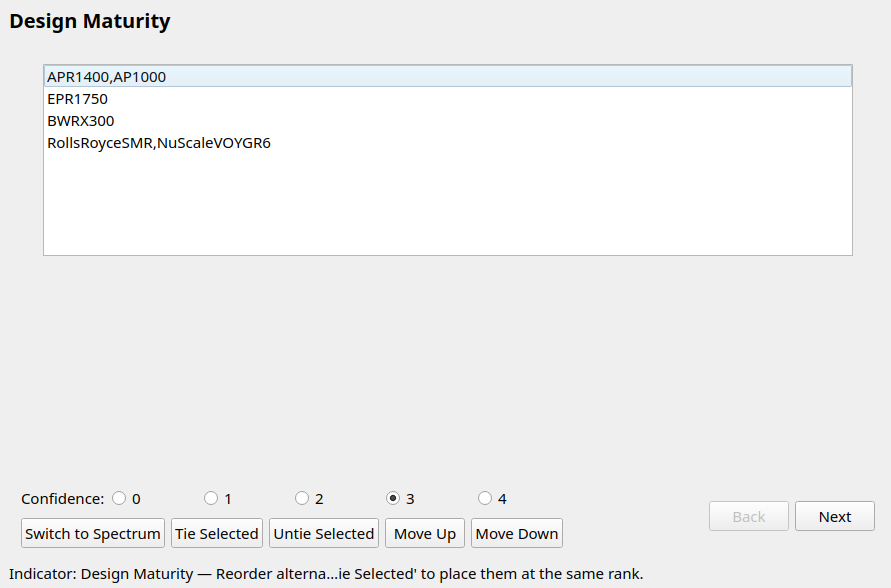
\includegraphics[width=\textwidth]{./imgs/QI_rank.png}
        \captionof{figure}{Ranking screen.}
        \label{fig:qi_order}
    \end{minipage}

    \vspace{0.75em}

    \begin{minipage}{0.85\textwidth}
        \centering
        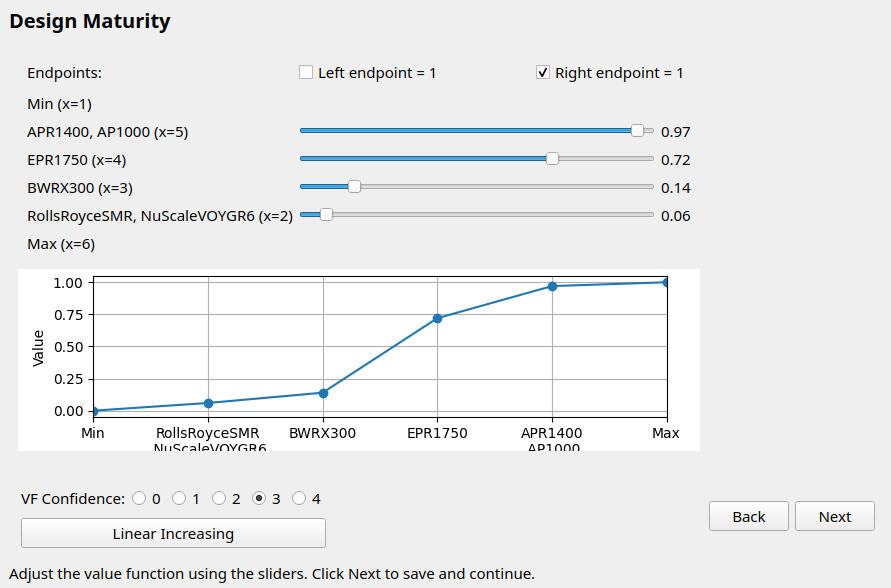
\includegraphics[width=\textwidth]{./imgs/QI_vf.png}
        \captionof{figure}{Value function screen.}
        \label{fig:qi_value}
    \end{minipage}
    \caption{Graphical interface for the elicitation of qualitative indicators.}
    \label{fig:qi_elicitation}
\end{figure}

\begin{figure}[htbp]
    \centering
    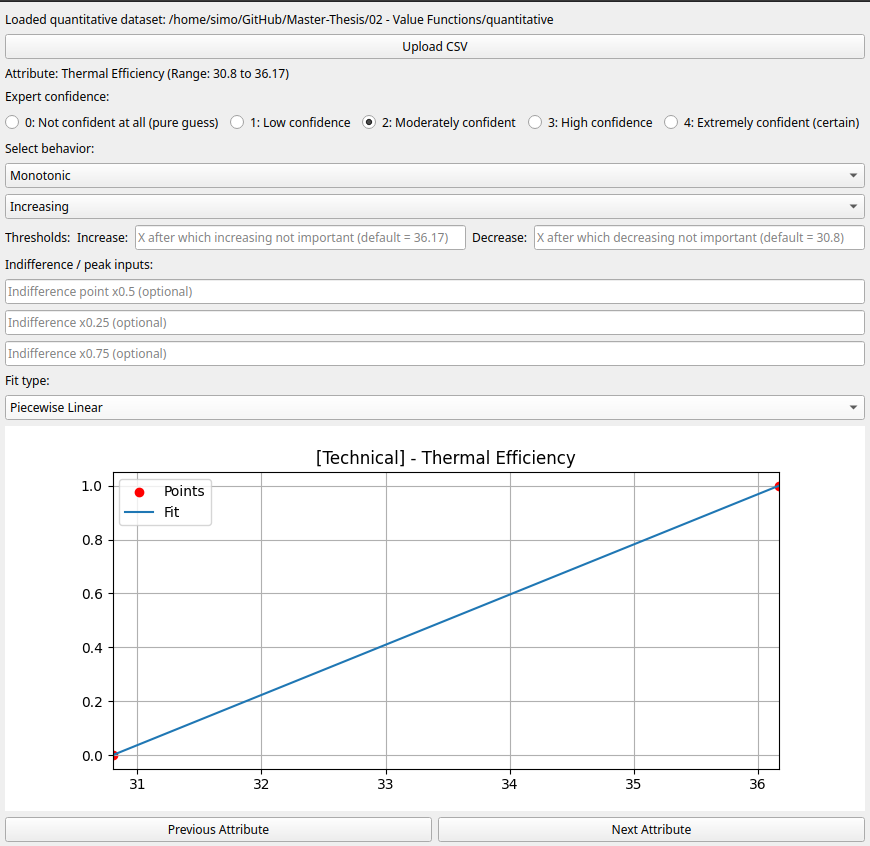
\includegraphics[width=0.75\textwidth]{./imgs/vf_UI.png}
    \caption{Value function elicitation interface showing mid-value splitting technique implementation.}
    \label{fig:value_function_elicitation}
\end{figure}

\begin{figure}[htbp]
    \centering
    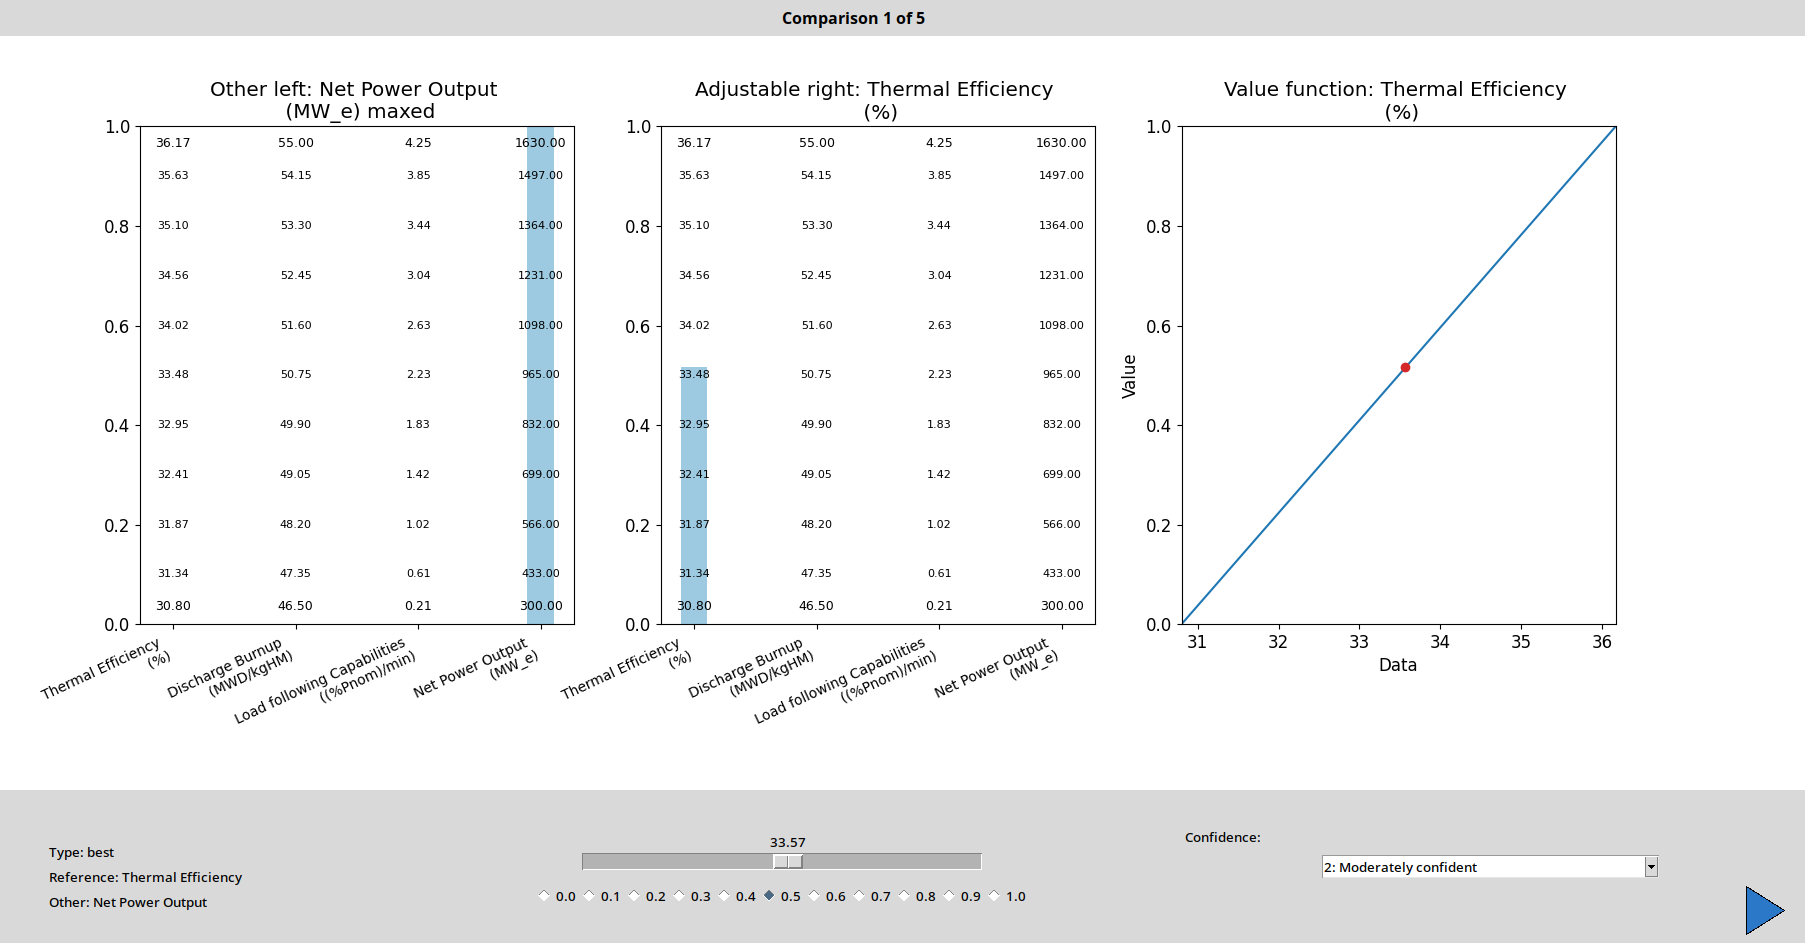
\includegraphics[width=0.8\textwidth]{./imgs/bwt_UI.png}
    \caption{Weights elicitation interface showing \gls{bwt} implementation.}
    \label{fig:weights_elicitation}
\end{figure} % Prentation of the Digital Tools developed to support the elicitation process

\chapter{Discussion and Results} % Post processing
\label{sec:final}
\section{Results of the analysis}
\label{sec:results}
This chapter reports results in three steps: elicitation inputs and outputs, uncertainty propagation through \gls{upmavt}, and final rankings. Only results are reported here; interpretation and methodological implications are discussed in Section~\ref{sec:discussion}.

\subsection{Elicitation inputs and outputs}

\subsubsection{Full elicitation sessions}
The elicitation process involved four experts who performed all analytical steps: (1) quantitative indicator value function development, (2) qualitative indicator assessment and value function construction, and (3) weight determination using the \gls{pilebwt} methodology. Expert backgrounds are summarized in Table~\ref{tab:experts}, identities are maintained confidential.

\begin{table}[htbp]
	\centering
	\begin{tabularx}{\textwidth}{|c|X|X|}
		\hline
			extbf{Expert} & \textbf{Area of Expertise} & \textbf{Experience}\\
		\hline
		E1 & Risk Assessment (Academia) & Senior Scientist\\
		E2 & Nuclear Safety (Academia) & Senior Scientist\\
		E4 & Nuclear Safety (Industry) & Junior Engineer\\
		E8 & Energy System Modelling (Academia) & PhD Student\\
		\hline
	\end{tabularx}
	\caption{Experts involved in the elicitation process.}
	\label{tab:experts}
\end{table}

\subsubsection{Quick elicitation results}
\label{sec:quick_elicitation_results}
To enhance qualitative indicator characterization, five additional experts participated in an abbreviated "quick elicitation" process focused exclusively on qualitative indicators assessment (step 2). This expert panel is presented in Table~\ref{tab:quick_experts}.

\begin{table}[htbp]
	\centering
	\begin{tabular}{|c|c|c|}
		\hline
			extbf{Expert} & \textbf{Area of Expertise} & \textbf{Experience}\\
		\hline
		E3 & Nuclear Plants (Academia) & Academic Professor \\
		E5 & Project Controlling for Nuclear (Industry) & 20 years in Project Managment positions \\
		E6 & Nuclear new Construction (Industry) & 17 years in Nuclear Construction\\
		E7 & Nuclear Plant Managment (Industry / EU) & 17 years in Nuclear Operations, currently working for EU JRC\\
		E9 & Probability Safety Assessment (Industry / UN)& 15 years in PSA for Nuclear related projects, currently working at IAEA\\
		\hline
	\end{tabular}
	\caption{Experts involved in the quick elicitation process.}
	\label{tab:quick_experts}
\end{table}

Figure~\ref{fig:quick_examples} illustrates the results for "Design Complexity", presented as a value heatmap to visualize the elcited values to each alternative across all experts.

\begin{figure}[htbp]
	\centering
	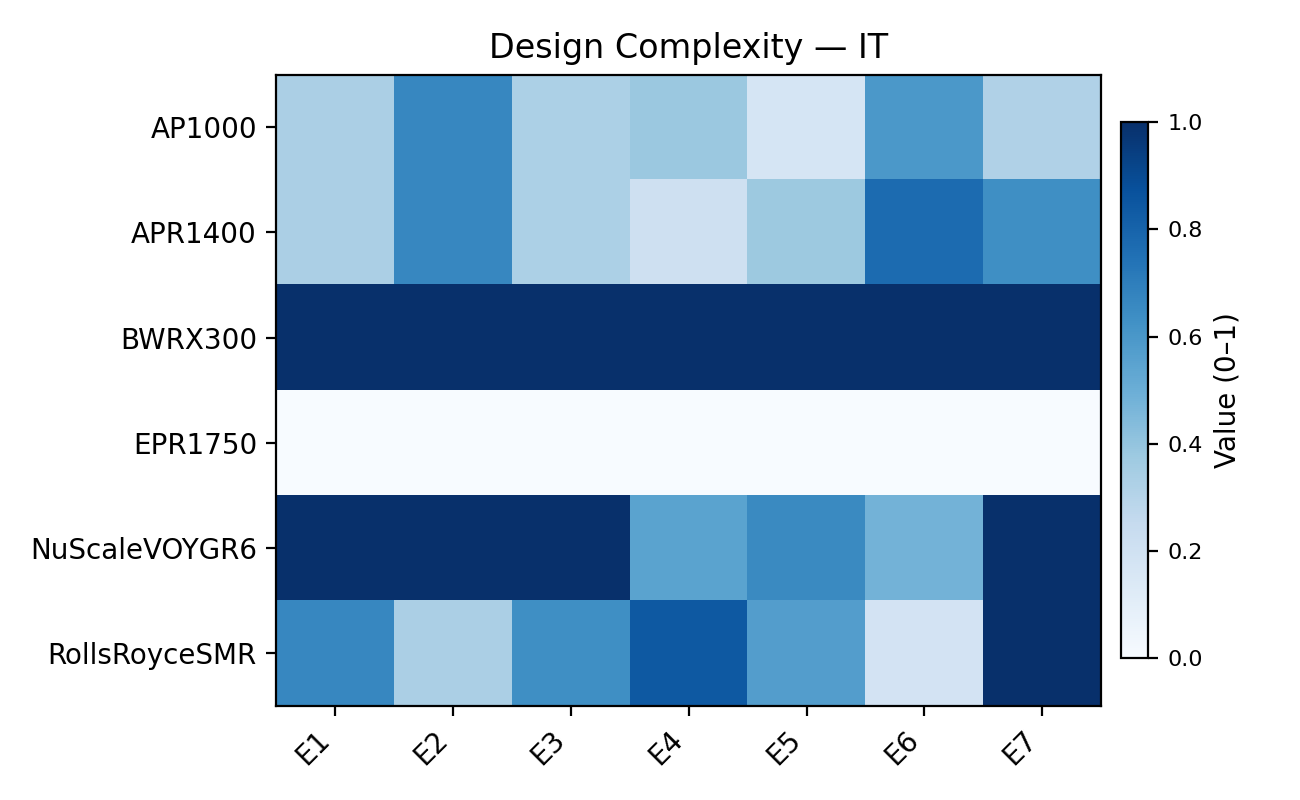
\includegraphics[width=0.75\linewidth]{imgs/QI_result_example.png}
	\caption{Values for the qualitative indicator "Design Complexity".}
	\label{fig:quick_examples}
\end{figure}

\subsubsection{Representative elicitation outputs}
Figure~\ref{fig:vf_examples} presents the value functions elicited from the four experts for the same indicator, showing the divergencies between expert opinions. Figure~\ref{fig:weight_space_results} shows weight elicitation outcomes presenting the feasible weight space, explored via differential evolution (SciPy implementation \cite{PLACEHOLDER}). Figure~\ref{fig:consistency_results} presents the consistency plots, which compare the declared pairwise comparison ratios with the ratios between the optimized weights. Each second bar represents the mean weight sampled from the feasible solution space, with error bars indicating $\pm \sigma$ to quantify solution variability. This adapted presentation, building on \cite{PLACEHOLDER}'s consistency analysis, explicitly incorporates uncertainty bounds from the weight space exploration.

\begin{figure}[htbp]
	\centering
	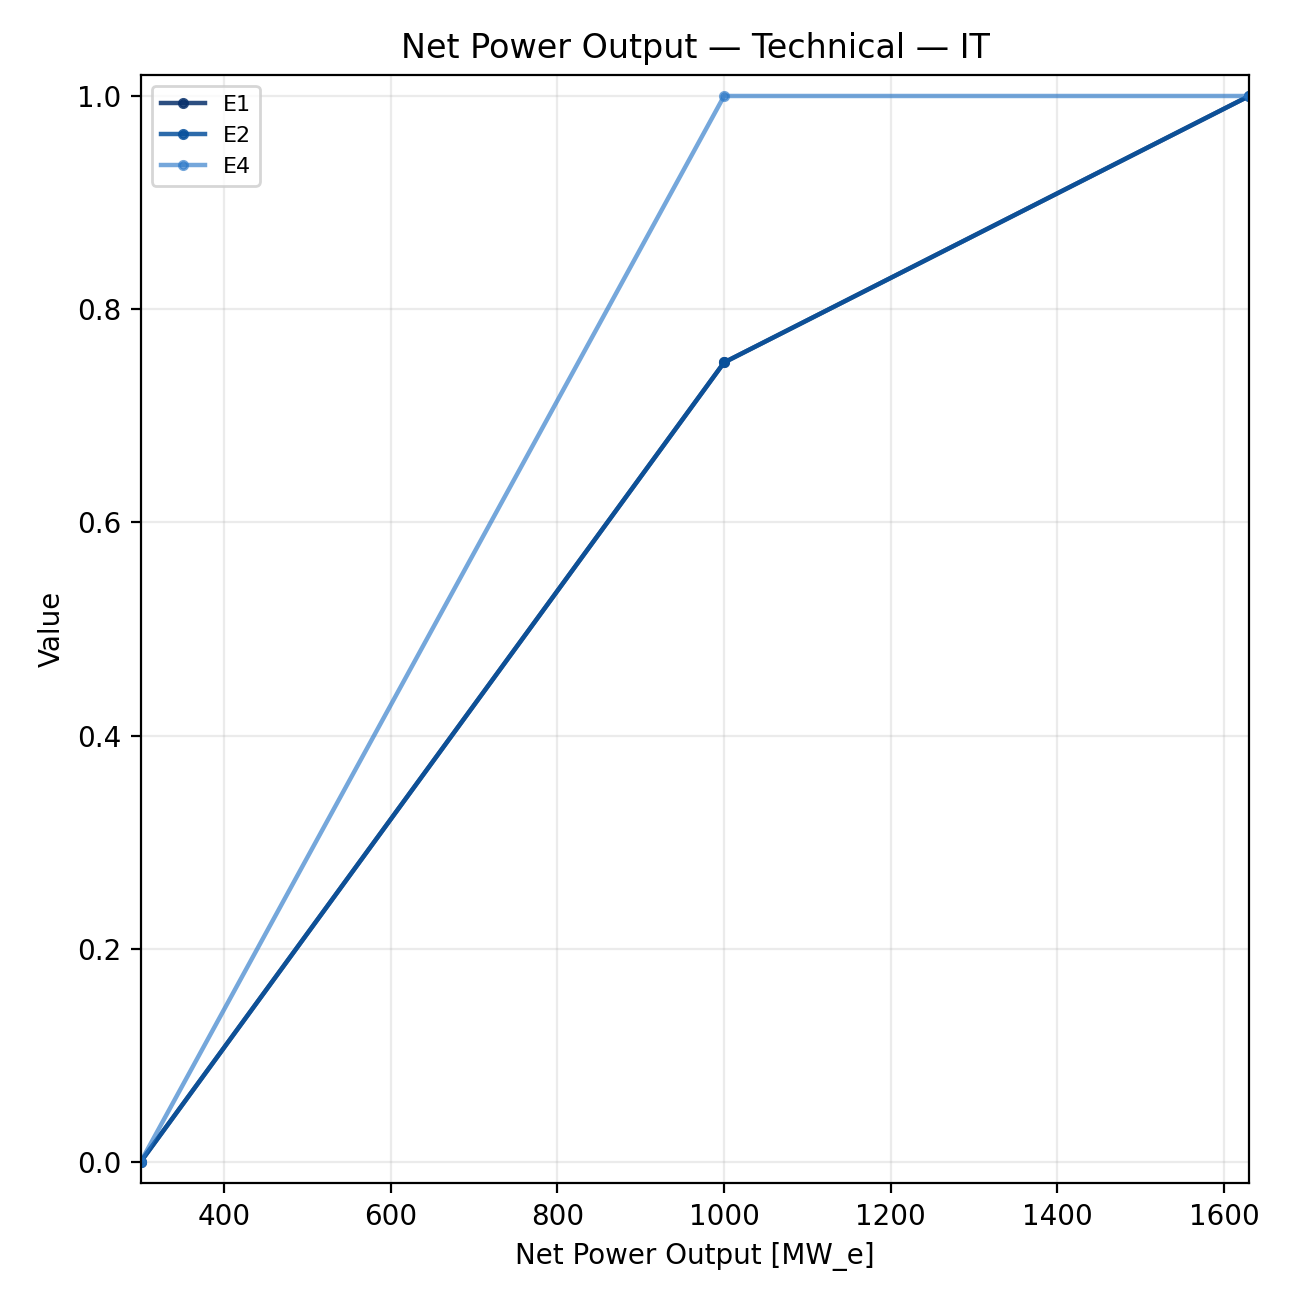
\includegraphics[width=0.5\linewidth]{imgs/vf_result_example.png}
	\caption{Value function elicited by experts for "Net Power Output - IT".}
	\label{fig:vf_examples}
\end{figure}

\begin{figure}[htbp]
	\centering
	
\includegraphics[width=0.95\linewidth]{weight_space_example.pdf}
	\caption{Weight plot space for expert E4.}
	\label{fig:weight_space_results}
\end{figure}

\begin{figure}[p]
	\centering
	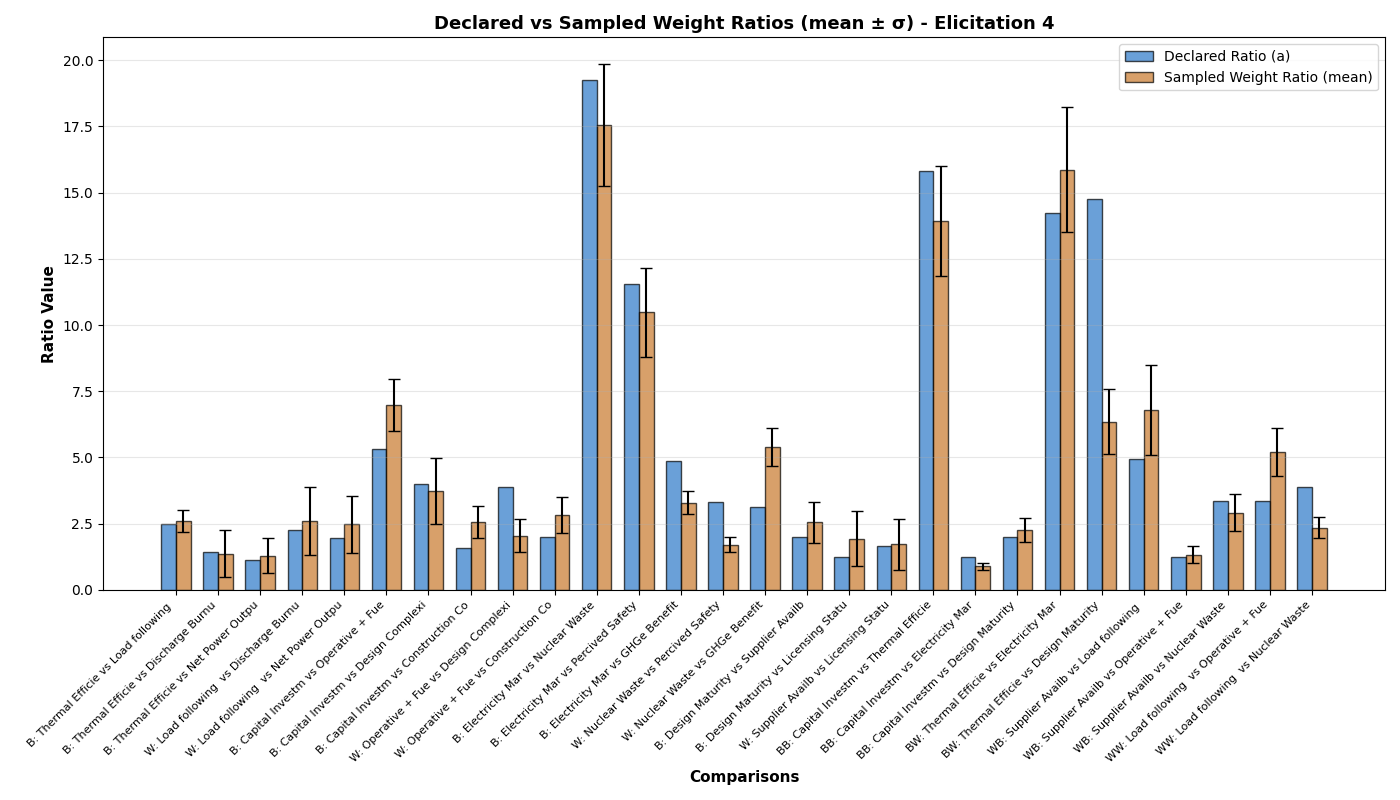
\includegraphics[angle=90,height=\textheight,keepaspectratio]{imgs/consistency_plot_example.png}
	\caption{Consistency plot for expert E4.}
	\label{fig:consistency_results}
\end{figure}

\subsection{UP-MAVT}
As established in Section~\ref{sec:uncertanty_propagation_mcda}, the \gls{smc} and \gls{nsmc} approaches serve complementary purposes. \gls{smc} results evaluate pre-aggregation uncertainty and expert consensus levels, while \gls{nsmc} generates final rankings. Representative outputs for one of the countries are presented in Figure~\ref{fig:smc_france_sum}, comparing weighted sum aggregation methodology.

\begin{figure}[htbp]
	\centering
	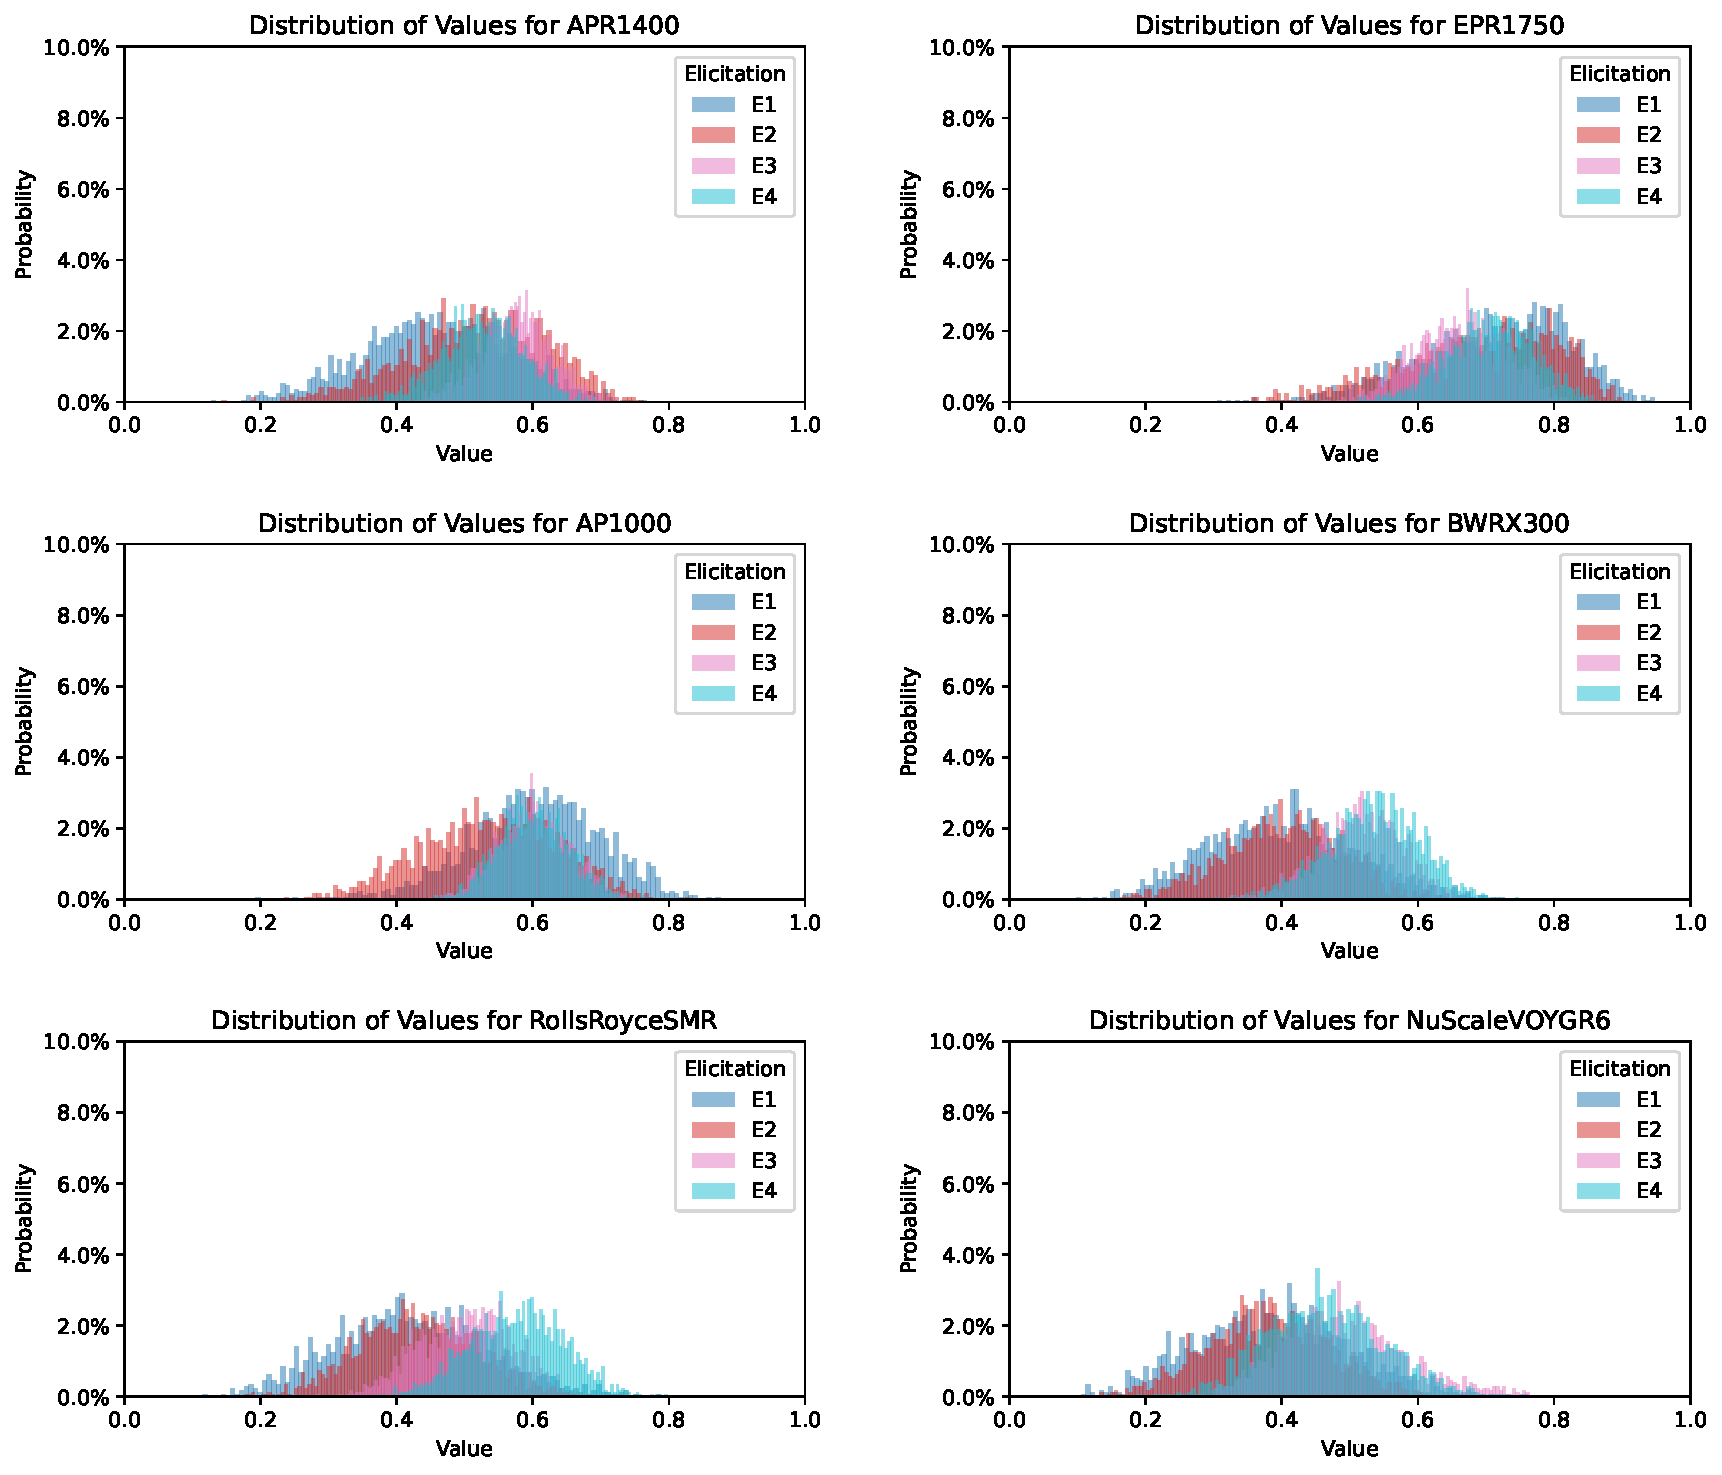
\includegraphics[width=0.95\linewidth]{Phase2_WeightedSum_Strict_FR_20260127_170138_histograms.pdf}
	\caption{\gls{smc} results for France using weighted sum aggregation (2000 iterations per expert).}
	\label{fig:smc_france_sum}
\end{figure}

\begin{figure}[htbp]
	\centering
	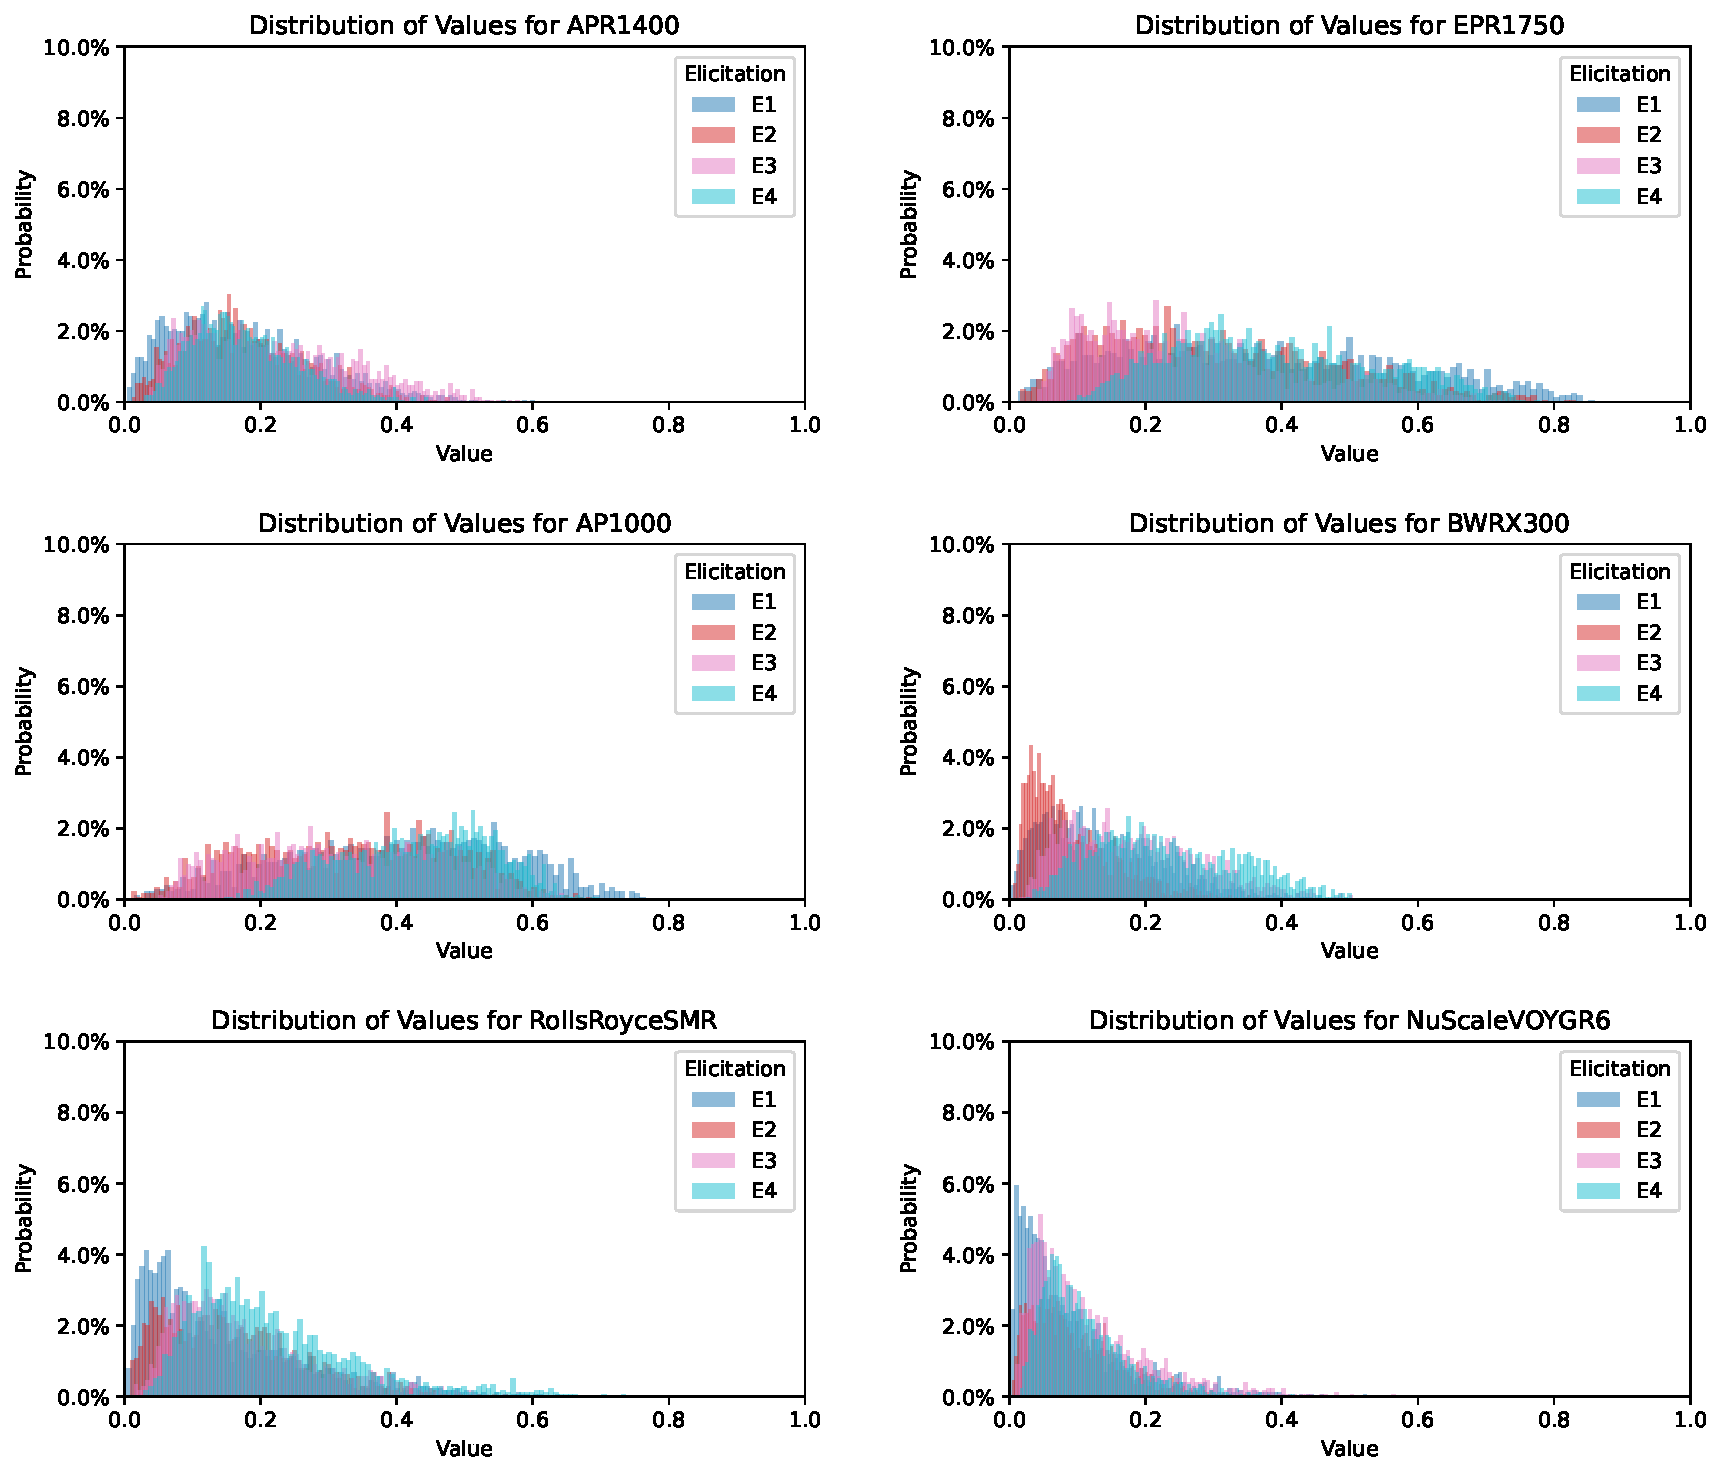
\includegraphics[width=0.95\linewidth]{Phase2_Geometric_Strict_FR_20260128_092214_histograms.pdf}
	\caption{\gls{smc} results for France using geometric mean aggregation, showing broader distributions and reduced dominance patterns.}
	\label{fig:smc_france_geo}
\end{figure}

\subsection{Rankings}
Ranking heatmaps are reported for each country across the three aggregation methods. Figures~\ref{fig:aggregation_methods_comparison_france}--\ref{fig:nsmc_rankings_po} present the \gls{nsmc} results using geometric mean aggregation for the country-specific summaries, alongside a cross-method comparison for France.

\begin{figure}[htbp]
    \centering
    \subfloat[\gls{sum}]{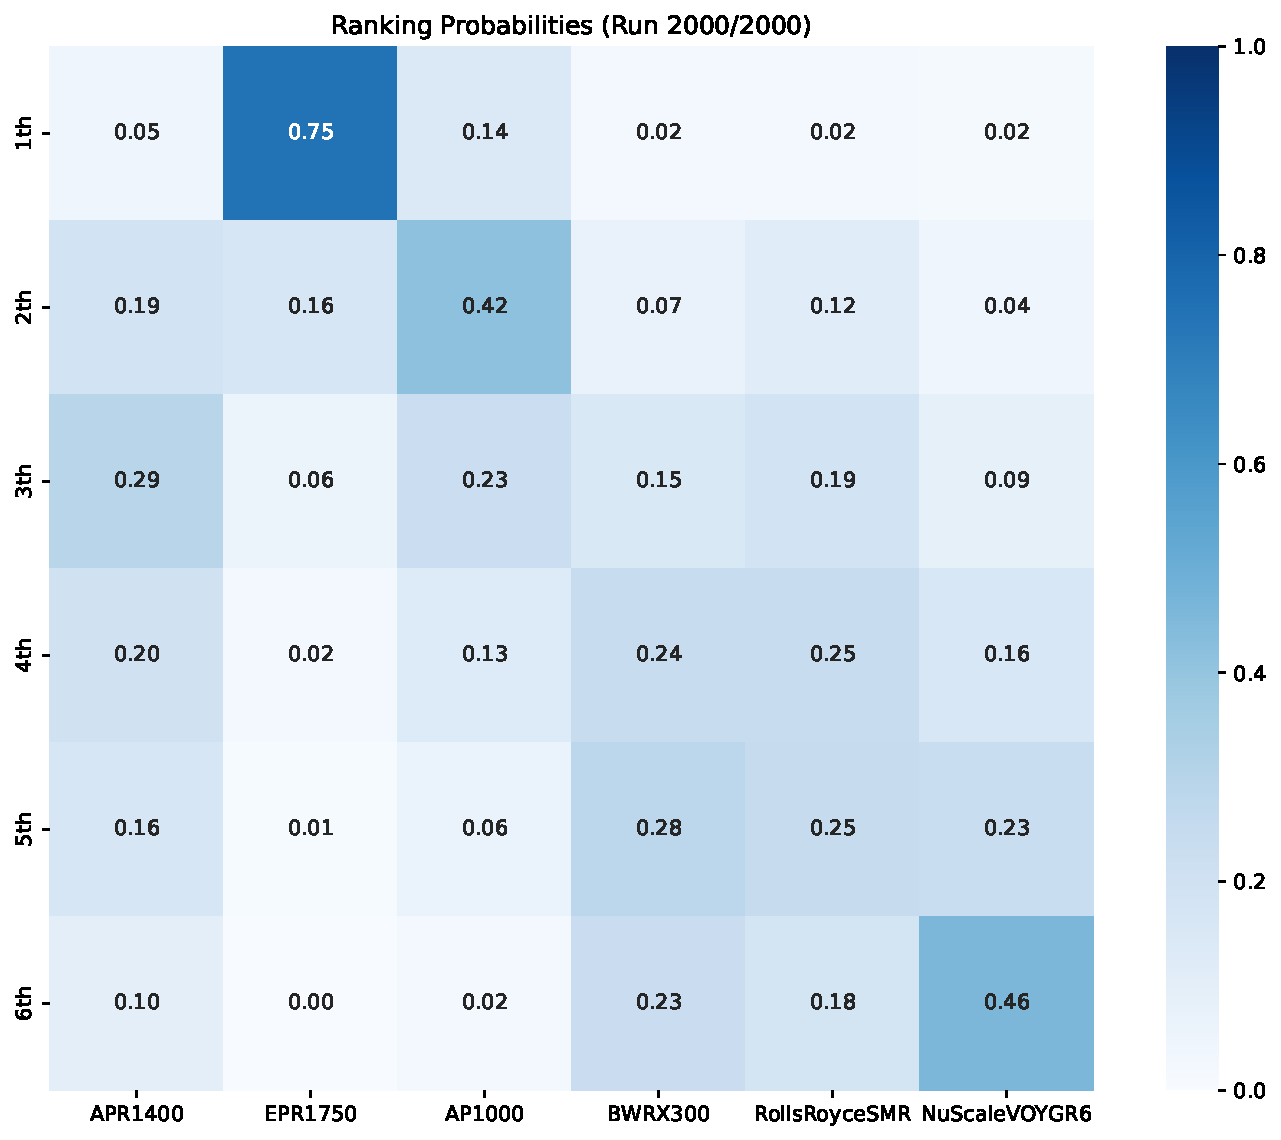
\includegraphics[width=0.32\linewidth]{Phase3_AllMethods_FR_weighted_sum_20260127_171441_heatmap.pdf}}\hfill
    \subfloat[\gls{geo}]{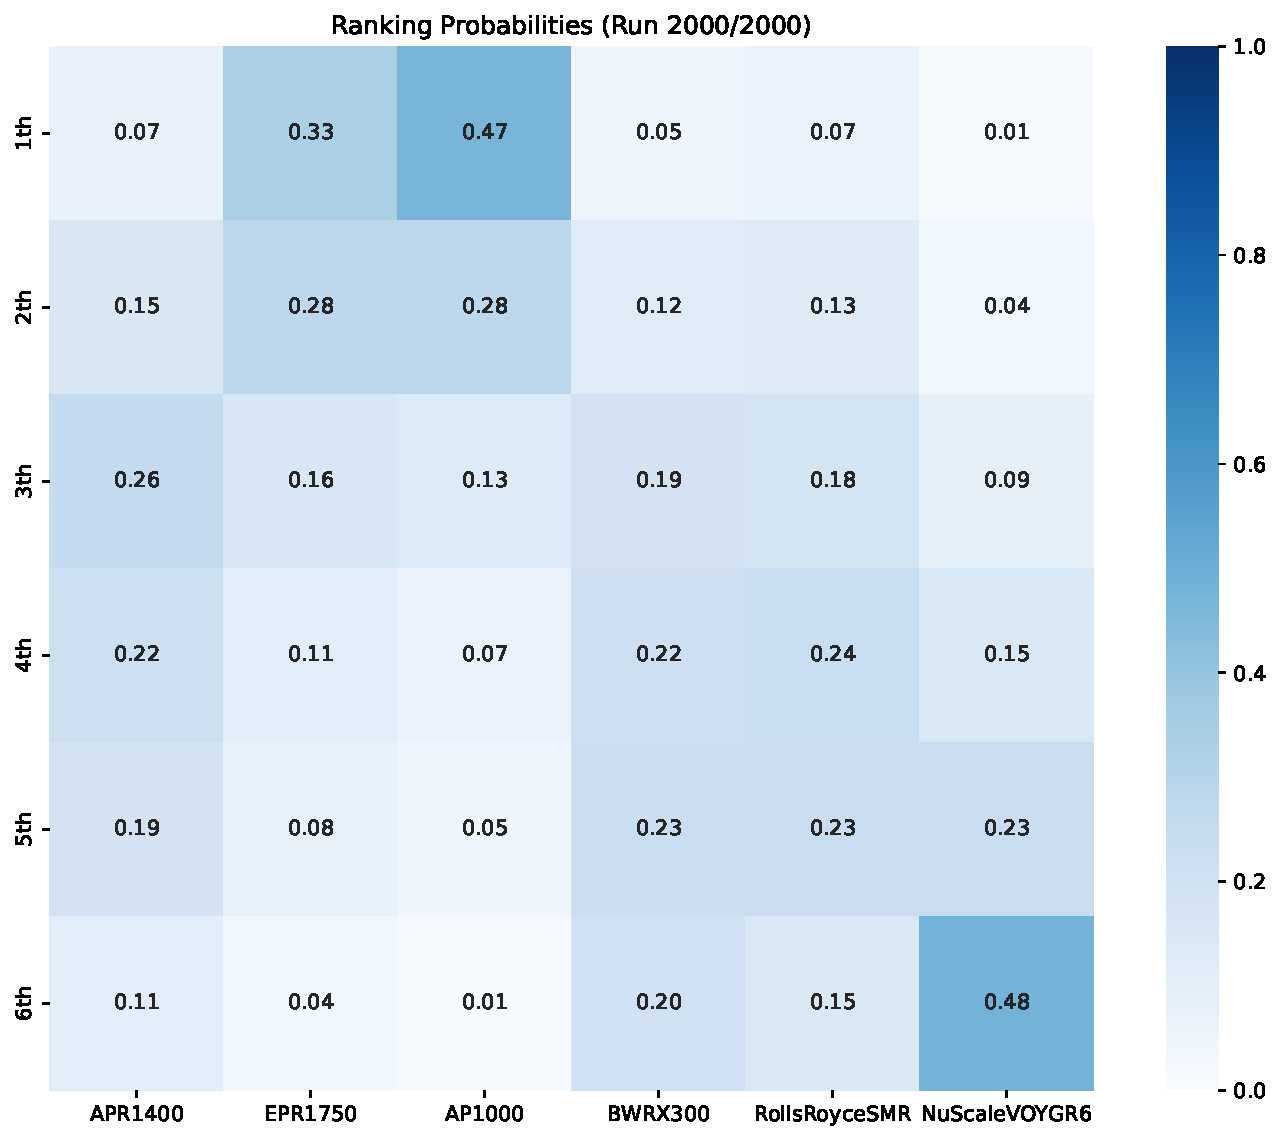
\includegraphics[width=0.32\linewidth]{Phase3_AllMethods_FR_geometric_mean_20260127_171648_heatmap.pdf}}\hfill
    \subfloat[\gls{har}]{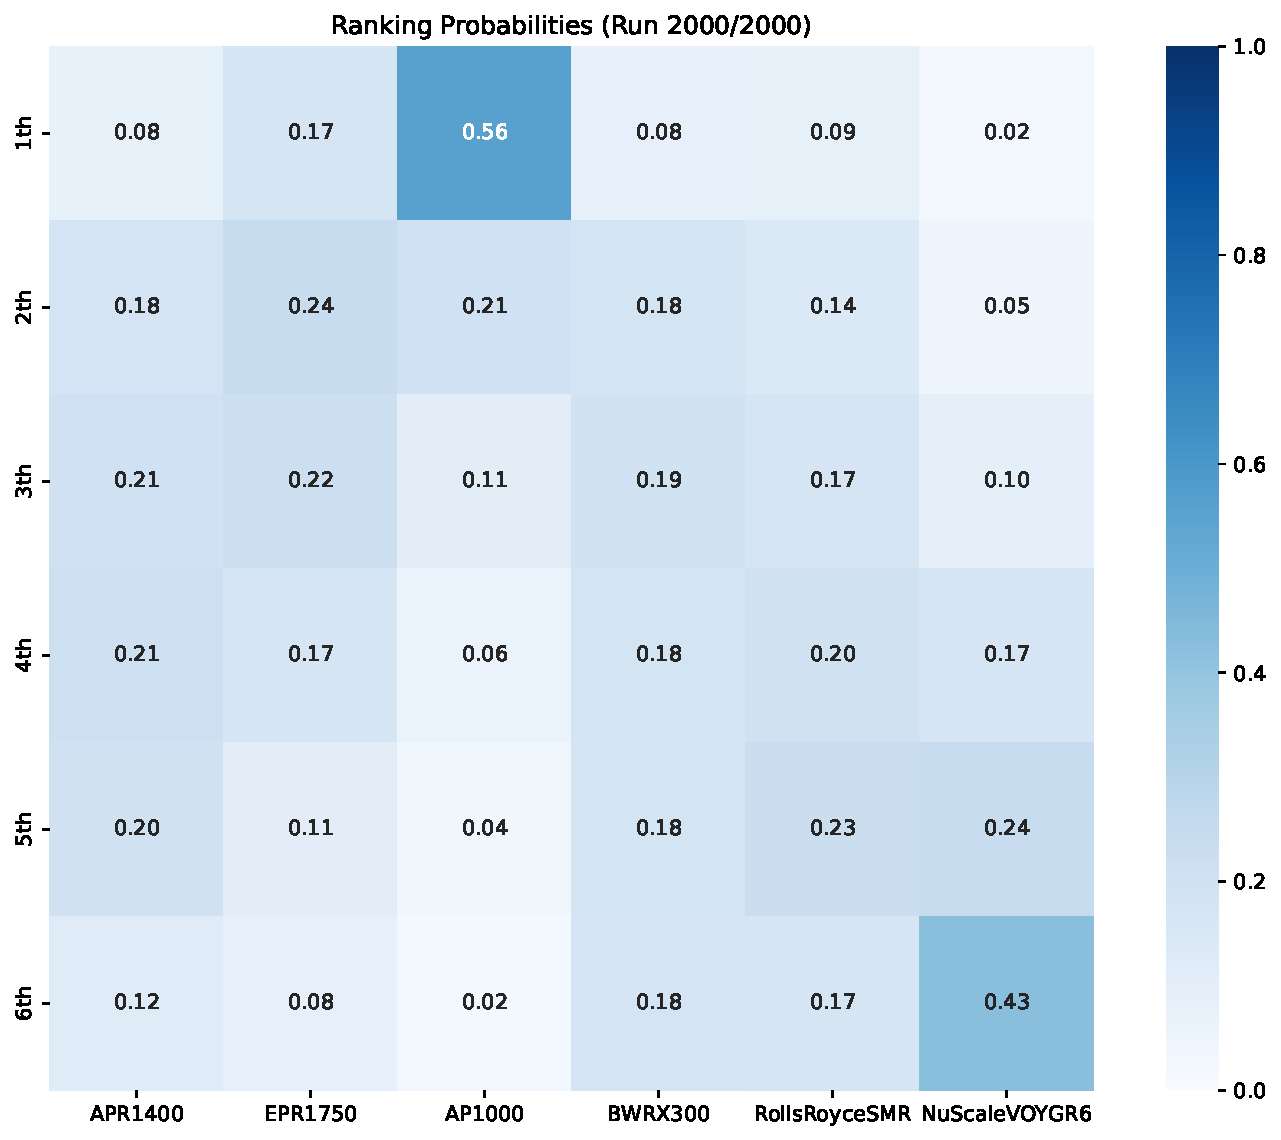
\includegraphics[width=0.32\linewidth]{Phase3_AllMethods_FR_harmonic_mean_20260127_171543_heatmap.pdf}}
    \caption{France: \gls{nsmc} ranking heatmaps obtained with different aggregation methods. Results show dominance of large reactor designs and ranking sensitivity to compensation method.}
    \label{fig:aggregation_methods_comparison_france}
\end{figure}

\begin{figure}[htbp]
    \centering
    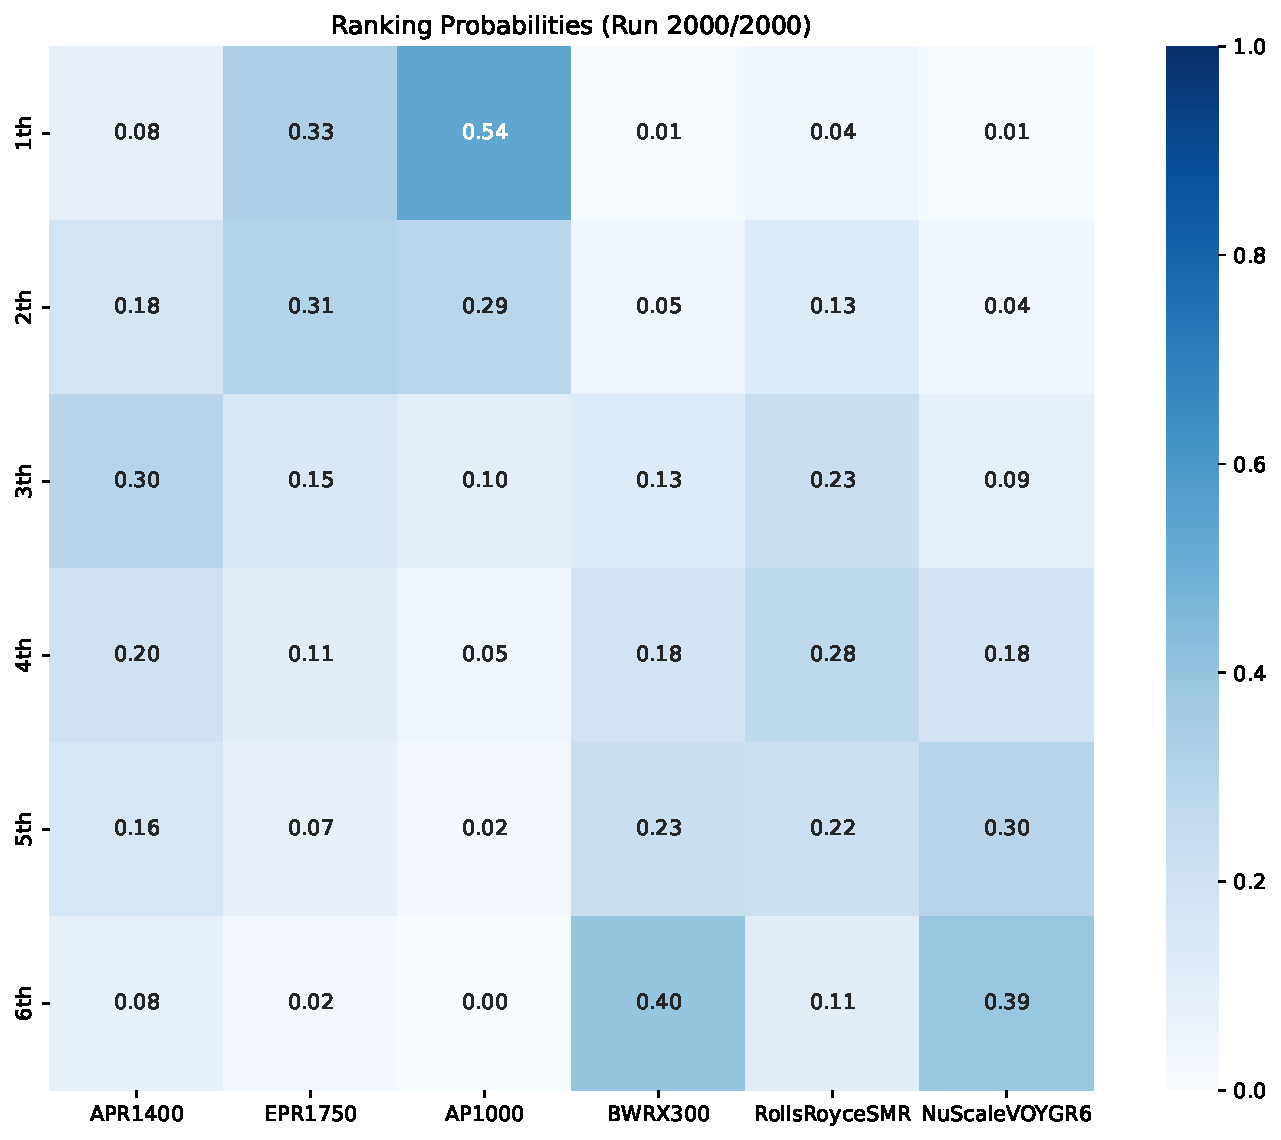
\includegraphics[width=0.95\linewidth]{Phase3_AllMethods_IT_geometric_mean_20260127_171336_heatmap.pdf}
    \caption{Italy: \gls{nsmc} ranking heatmap with geometric mean aggregation.}
    \label{fig:nsmc_rankings_it}
\end{figure}

\begin{figure}[htbp]
    \centering
    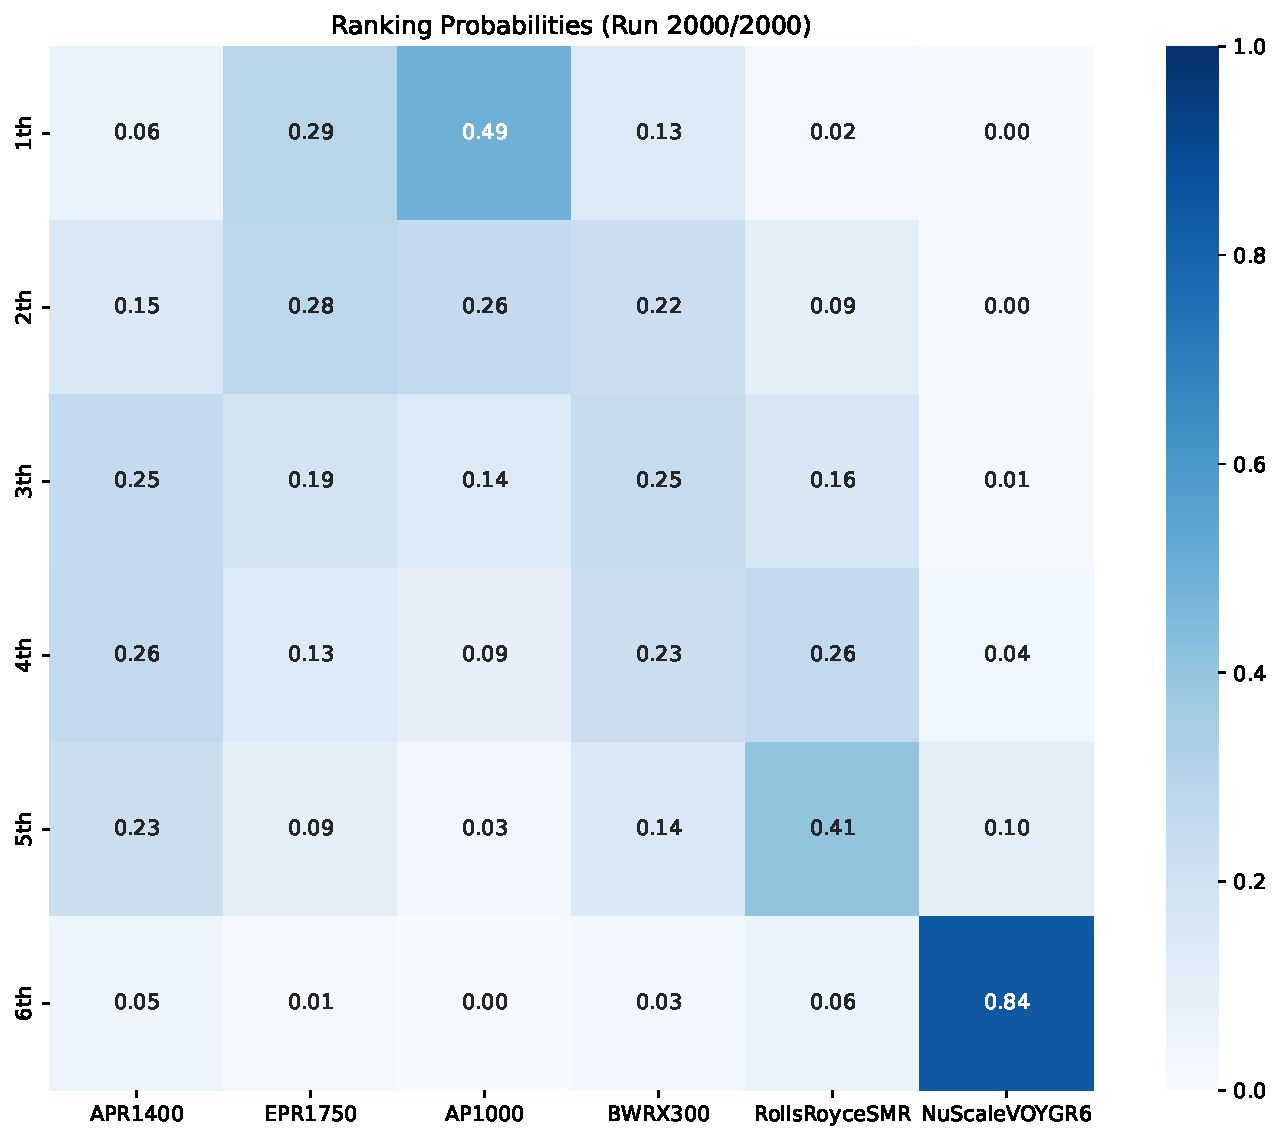
\includegraphics[width=0.95\linewidth]{Phase3_AllMethods_CH_geometric_mean_20260127_172000_heatmap.pdf}
    \caption{Switzerland: \gls{nsmc} ranking heatmap with geometric mean aggregation.}
    \label{fig:nsmc_rankings_ch}
\end{figure}

\begin{figure}[htbp]
    \centering
    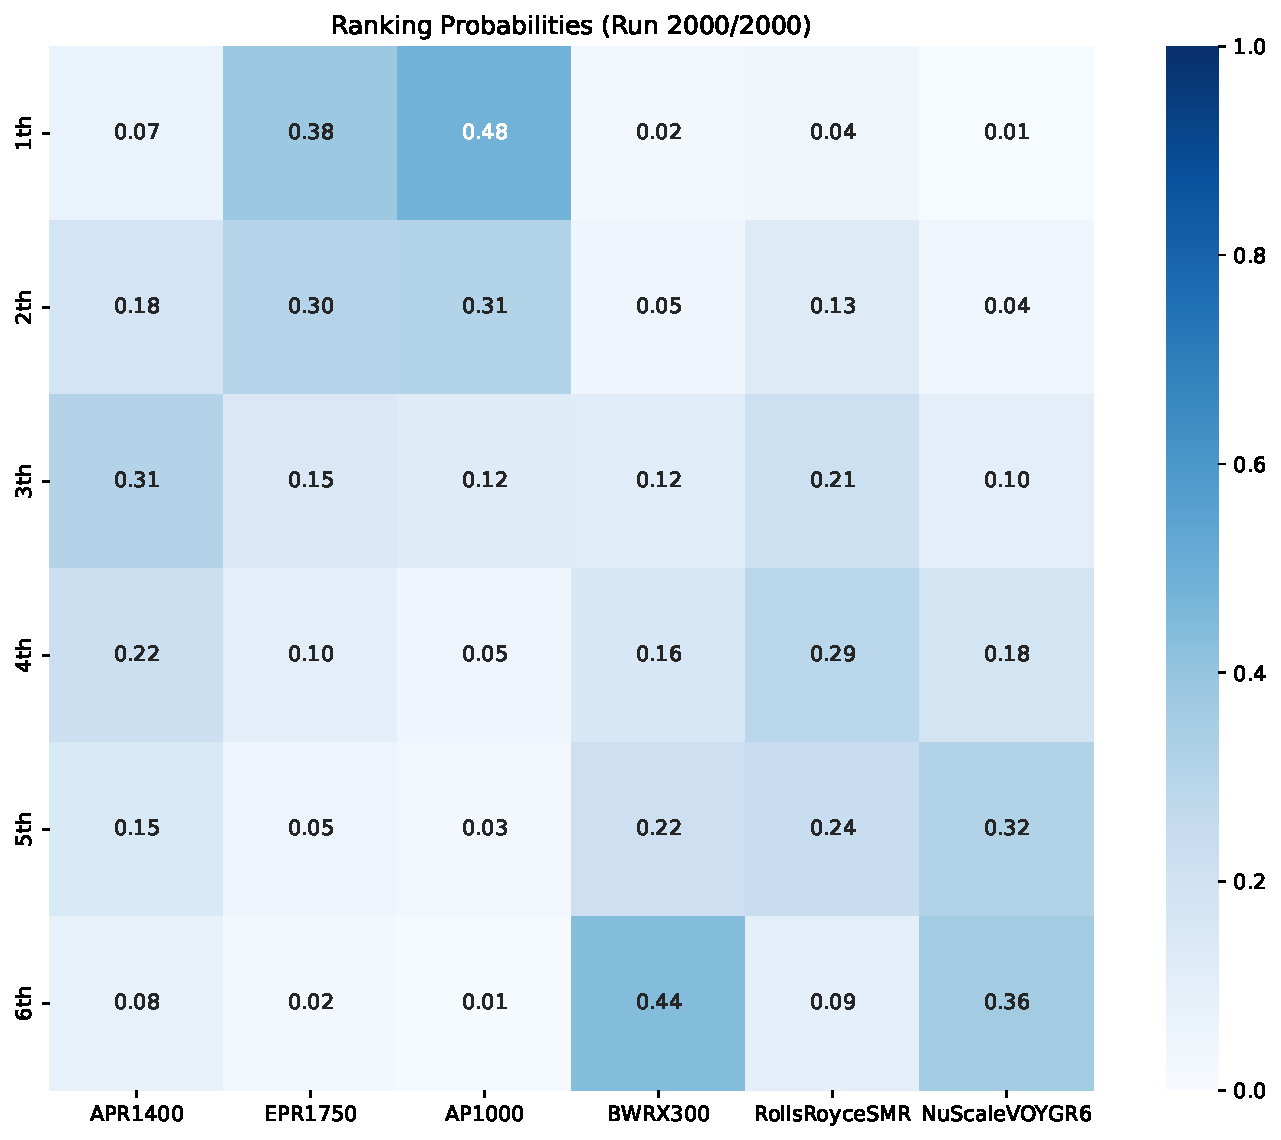
\includegraphics[width=0.95\linewidth]{Phase3_AllMethods_PO_geometric_mean_20260127_172306_heatmap.pdf}
    \caption{Poland: \gls{nsmc} ranking heatmap with geometric mean aggregation.}
    \label{fig:nsmc_rankings_po}
\end{figure}

 % Results of the analysis
\section{Discussion}
\label{sec:discussion}

\subsection{Elicitation}
The "first elicitation" session took noticeably more time than the others at 3 and a half hours. The following sessions all took no more than 2 and a half hours, showing that, as predicted in Sections~\ref{sec:value_functions} and~\ref{sec:qualitative_indicators_uncertainty}, the use of a first elicitation as a starting point for the following ones sped up the process considerably. An important aspect to discuss is the way the \gls{pilebwt} elicitation was carried out: in principle the comparison should have been reperated for each country beacuse of the intrinsic importance of the range of data for each indicator, which differ in this analysis, for example the "Electrcity amrket benefit" is a country-dependant indicator. However, to limit the required time the comparisons were always carried with a range that included the minimum and maximum data points across all countries. After the elicitation the elicited data point of a comparison was trasposed to the specific country range by means of linear mapping. This ensures that the country dependent value functions are still meaningul when applied to such data value, something that could not be possible if the transposition was to assume a non linear mapping, or if it was to just clip the values to the country range. To the author's knowledge, this approach should not introduce any significant bias in the results, however, further analysis could be carried out to confirm this assumption.

\subsection{Inconsistency Management}
Regarding the weighting process, expert E3 was extremely consistent in their judgments, helped by the fact that they were experienced in the use of \gls{mcda} methods. The other experts showed a varying degree of inconsistency, with expert E1 showing the highest inconsistency. As anticipated in \ref{sec:results}, expert E1 was very inconsistent in their \gls{pilebwt} judgments, however, the results obtained show that even including their input does not drastically change the final ranking, although, as expected, it does increase the uncertainty in the results.

Due to the nature of the \gls{pilebwt} method whcih has to be solved by means of optimization models, it was observed that inconsistencies in the judgments would prevent obtaining satisfactory results. Only cardinal consistency was considered in this analysis, that is, the order of the indicators cannot change between best comparisons and worst comparisons. For experts E2 and E4, some of these inconsistencies existed by a very low margin and were therefore corrected by slightly modifying the judgments. For example, the declared value by the expert in a comparison was 0.40, but to ensure consistency, it should have been greater than 0.45; the analysts adjusted the value to 0.45. For expert E1, some inconsistencies were much more severe and could not easily be corrected. However, the \gls{pilebwt} optimization model managed to run anyway, producing a wider weight space. To obtain the results of this thesis, both the results by excluding expert E1 and including them are shown, to demonstrate the effect of such inconsistent judgments on the final ranking.

\subsection{Observations on Expert Perspectives}
Thoughout the elicitations session it was clear that expert opinions were mostly aligned in their basis of judgment but ultimatly differed in the conclusions due to their different knowledge. This was expecially evident in the \glspl{qi} elicitations, where experts were more free to express their opinions. Context information in this regard proved to be the critial braking point between experts, for example, some experts would consider a certain licensing status as very good due to their knowledge of the technology, while those aware of political matters that affect some countries would rate the same status lower. This highlights the importance of selecting experts with diverse backgrounds to capture as many perspectives as possible. In the judgment of \glspl{smr} "insider" knwoledge was found to influence deeply the final outcome, were most would rate a technology at a certain level, the expert with direct experience with the same technolgy rated it lower due to their knowledge of recent issues that are not well known, even within the industry.

Regarding the \glspl{qi} themselves, the most critiqued one was the "design complexity" as many experts considered that it was possible to quantify it fairly easily by considering the number of safety systems, modularity level, redundancy level, etc. Second the "Construction Complexity" that the current study presented as country dependent was considered by most experts to be rather "country agnostic", as construction complexity would be mostly driven by the design itself rather than the country specific factors. Regarding "Construction Complexity", the author starting point was not preferring any design due to the belif that off-site construction and modularity do not bring a clear advantage in practice. All experts agreed on this viewpoint, mentioning that while modularity is, on paper, beneficial, it is yet to be proven and it is most likely to face several issues in their first of a kind projects.

All experts brough at some point in the conversation the significant influence that politics has on nuclear projects, behiond commitment, the ultimate choice of a reactor model is often driven by political factors and international relations rather than technical or economic merits. While this aspect is hard to quantify, it is important to acknowledge its role in the decision-making process for nuclear new builds.

Industry consultations revealed significant skepticism about SMR feasibility, primarily concerning vendor transparency. Experts questioned SMRs' market relevance, noting that most countries prioritize large-scale replacements for retiring capacity (e.g. replacement of coal-fired power plants in Poland). While the EPR's 1600 MWe capacity exceeds many nations' needs, the consensus identified 1000-1400 MWe as the optimal range for national deployment. SMRs were seen as potentially viable for private investors seeking smaller integrated solutions, but less suitable for utility-scale projects.

The proliferation of competing SMR designs was identified as problematic, creating decision paralysis for national entities while confusing public perception. Some observers suggested certain projects might represent "paper reactors" primarily aimed at securing funding rather than achieving commercial deployment. % Discussion and comments on the results
\section{Suggestions for further improvements and extensions}
\label{sec:suggestions}
Here we suggest possible improvements and extensions to this thesis:

\subsection{Improvements on the Case Study}
For some indicators we decided to "play it safe" by using today's data. For a more indicative analysis it coluld be interesting to implement forecasts for emissions, costs and electricicty prices and demands.
Improvement of the risk of delay indicator by providing a risk assesment analysis. Same thing goes for the feasibility indicators that would require more in depth analysis.

If a siting approach was to be implemented as well, we suggest the following indicators
- Impact on landscape (social)
- Impact on the grid (technical)
- Proximity to energy demand (technical/economic)
- Local Job creation potential (social)
- Economic development potential from a national point of view (economic)
- Proximity to useful industry (for the commissioning itself)

If a siting approach is used then a group for enviromental concerns but that should be ocnsidered as the point of view of the agencies in charge of enveriomental assesment NOT FROM THE POV OF THE PUBLIC:
- water usage and impact on local water systems
- land use (considerig what the land was used for before the plant construction)
- accompanying infrastructures needed (means further land use that can be considered without a deep enviromental analysis but from a more qualitative point of view to simplify the analysis)
Impact on local biodiversity is not a good indicator since we assume that the siting process would start from a set of reasonable sites, excluding protected areas and areas of high biodiversity value.

For a national level analysis could be interesting to consider an objective such as reducing imports so that the analysis is focused on deployment solutions, for instance 1 EPR vs 5 SMRs to conver the same energy demand.

\subsection{Improvements on the Elicitaiton process}
The greatest improvement that can be suggested to improve the elicitation process is to implement an interactive software that allows for remote elicitations session, that do not require the attendance of the analysis and that would allow the expert to perform the elicitation at their own pace. This would reduce the burden on both the experts and the analysts, allowing for more experts to be involved in the process and therefore improving the quality of the results.

Regarding the methodology used, as expected the "first elicitation" followed by "corrections" was of great help in speeding up the process. For value functions it was found very limiting to force experts to use the indifference points that were defined from the mid-splitting technique in the first elicitation, it is therefore suggested to allow experts to more free adjustment of the points in the following elicitations. In the \gls{qi} elicitation the use of a "standard" reference alternative was found to be very useful, and it is suggested to keep using it in future elicitations, the use of a "spectrum" instead of ranking in the starting point of for "construction complexity" (See section \ref{sec:economic_indicators}) was found to be very confusing for the experts and therefore it is suggested to avoid this approach in future elicitations. Regarding the \glspl{qi} eliciations the author suggest to explore the possibility to involve multiple experts at once in a group elicitation so that they can discuss and share their perspectives, in multiple instance it was found that experts might miss details that were obvious to others, for this reason group elicitations might be of great help in improving the quality of the results.

Finally on regard of the \gls{pilebwt} elicitaiton method, the use of a UI to help experts was of great help, guidance thoughout this process is still very likely to be necessary to force experts into proper use of the method, otherwise a very extensive and comprehnsive tool would be needed to properly guide them. The method was deemed difficult form the experts not beacuse difficult to understand but because of the intrinsic difficulties in quantivy a pairwise comparison, for this reason it is suggested to keep in mind the high cognitive burden of this task when planning the elicitaiton sessions. Moreover it was very easy for experts to "cheat" the method by providing values based on "how much more important is A then B" instead of aswsering the proper methodlogically accurate question: "How much do I have to increase A form its minimum to compensate for the decrease of B from its minimum to its maximum", for this reason it is suggested to stress the difference between the two approaches when explaining the method to experts.

\subsection{Improvements on the \gls{upmavt} method}
First and foremost, the author suggests to further investigate the use use of Uncertanty Progpagation in MCDA methods, extending the UP- approach to other MCDA methods. A feature that was not implemented, mostly to limit the burden of this thesis work, was a system of uncertanty tracking, which could be accomplished by carefully recoding each step of the \gls{upmavt} process to keep track of the uncertanty sources thoughout their propagation. This could be useful to identify which steps, indicators or experts contribute the most to the overall uncertanty, and therefore help in focusing future efforts to reduce it. % Suggestions for further improvements and extensions


%-------------------------------------------------------------------------
%	BIBLIOGRAPHY
%-------------------------------------------------------------------------
\nocite{*} % Example citation to avoid compilation errors :D
\printbibliography

%-------------------------------------------------------------------------
%	APPENDICES
%-------------------------------------------------------------------------

\cleardoublepage
\addtocontents{toc}{\vspace{2em}} % Add a gap in the Contents, for aesthetics
\appendix
\chapter{Code Appendix}
\label{sec:appendix_code}

All computational materials supporting this research are available in the following GitHub repository:
\url{https://github.com/simo-pagliu/Master-Thesis/}

The repository contains:
\begin{itemize}
    \item \textbf{Reactor Selection and Analysis}: Implementing the methodology described in Section \ref{sec:selection_reactors} (Location: \texttt{01\ -\ Attributes\ Definition/Reactors\ Data/Reactor\ Analysis.ipynb})
    \item \textbf{Energy Data Analysis}: Supporting the country selection process outlined in Section \ref{sec:country_selection} (Location: \texttt{01\ -\ Attributes\ Definition/Electricity\ Data/Electricity\ Market\ Analysis.ipynb})
\end{itemize}

\chapter{Perceived Safety Survey}
\label{sec:appendix_survey}
The survey prototype (Table \ref{tab:nuclear_survey}) illustrates a methodological approach for potential UP-MAVT integration, though the limited sample size (N=50) restricts statistical significance. The first question classifies respondents into a three tiers (pro-nuclear, anti-nuclear, neutral) that, while necessarily simplistic, reflects the binary nature of actual referendum decisions (yes or no). This categorization helps distinguish between respondents with fixed positions and those that are potentially more influenced by campaign messaging.

The second question establishes a baseline nuclear perspective, as the study focuses on relative comparisons rather than absolute judgment. Questions 3-5 present each manufacturer claims about their own SMR designs, emphasizing opinion formation dynamics over searching for an objective truth.

Demographic data collection includes age brackets designed to differentiate between those with firsthand memory of major nuclear accidents (Chernobyl/Fukushima) and those without, considering both voting age requirements and early childhood recollections (down to age 6).

Preliminary findings indicate that both neutral and pro-nuclear respondents slightly favor BWRX-300 and NuScale designs when compared to traditional reactors. The anti-nuclear subgroup (n=4) remains too small for meaningful analysis. A larger sample would enable further analysis of demographic patterns and correlations with initial attitude (Q2).




\begin{table}[h]
\centering
\caption{Public Perception of Nuclear Reactor Safety Survey}
\label{tab:nuclear_survey}
\begin{tabular}{>{\raggedright\arraybackslash}p{0.4\textwidth} >{\raggedright\arraybackslash}p{0.5\textwidth}}
\toprule
\textbf{Question} & \textbf{Response Options} \\
\midrule
What is your overall opinion on using nuclear power? &
\( R_1 \in \{\text{I strongly disagree}, \text{I do not hold any strong position}, \text{I strongly agree}\} \) \\

What is your opinion on the safety of traditional nuclear power plants? &
\( R_2 \in \{\text{Unsafe}, \text{Neutral}, \text{Safe}\} \) \\

Do you think the Rolls-Royce SMR is...? &
\( R_3 \in \{\text{Safer than traditional reactors}, \text{Indifferent}, \text{Less safe than traditional reactors}\} \) \\

Do you think the NuScale design is...? &
\( R_4 \in \{\text{Safer than traditional reactors}, \text{Indifferent}, \text{Less safe than traditional reactors}\} \) \\

Do you think the BWRX-300 is...? &
\( R_5 \in \{\text{Safer than traditional reactors}, \text{Indifferent}, \text{Less safe than traditional reactors}\} \) \\

What is your age group? &
\( R_6 \in \{\text{Under 20}, \text{Between 21 and 44}, \text{Over 45}\} \) \\

Where are you from? &
\( R_7 \in \{\text{Italy}, \text{Switzerland}, \text{France}, \text{Poland}, \text{Other}\} \) \\

How much do you know about nuclear power? &
\( R_8 \in \{0, 1, 2, \dots, 10\} \), where 0 = I know nothing, 10 = I'm an expert \\

Suggestions or comments? &
Open-ended response \\
\bottomrule
\end{tabular}
\end{table}


\chapter{Suggestions for Practitioners}
\label{sec:appendix_suggestions}
In this appendix suggestions to practitioners planning to carry similar studies are collected. These suggestions are based on the author's experience during the development of this thesis, shared hoping to facilitate future works in this field.

\subsubsection{Knowledge sharing sessions}
Elicitation sessions revealed fundamental alignment in expert judgment frameworks, with divergences emerging primarily from differences in thier specialized knowledge. This pattern was particularly pronounced in \gls{qi} assessments, where experts enjoyed greater interpretive freedom. Contextual awareness proved decisive: technological specialists often rated licensing statuses more favorably than colleagues attuned to country-specific political realities.

The \gls{smr} evaluations demonstrated how "insider" knowledge significantly influences outcomes. While most experts assigned similar baseline ratings, those with direct technology experience consistently applied more conservative assessments, reflecting awareness of recent, not well known, operational challenges. This underscores the value of multidisciplinary expert panels that incorporate both technical and contextual perspectives.

For these reasons, future studies should consider implementing knowledge-sharing sessions prior to individual elicitations. Such pre-elicitation exchanges would allow experts to present case-specific insights, potentially reducing deviations that stem from information asymmetries rather than genuine differences in professional judgment. This approach maintains individual assessment integrity while ensuring all experts operate from a common factual baseline.

\subsubsection{Methodological adherence in PILE-BWT elicitation}
During the \gls{pilebwt} elicitation, experts frequently defaulted to intuitive importance comparisons ("How much more important is A than B?") rather than the required compensatory trade-off formulation ("How much must A improve from its minimum to offset B's decline from minimum to maximum?"). Future applications must emphasize this distinction during expert briefings to maintain methodological rigor.

\subsubsection{Flexibility in value function correction}
During value function elicitation, when experts were asked to adjust the results of the "first elicitation", the rigid adherence to pre-defined indifference points from initial mid-splitting created unnecessary constraints. Future implementations should permit greater expert flexibility in adjusting these reference points during subsequent sessions.

\subsubsection{Possible improvements on QI approaches}
Regarding \glspl{qi} the use of a standardized reference alternative significantly improved consistency and is recommended for future studies. On the other hand, the "spectrum" approach for the "construction complexity" indicator (Section~\ref{sec:economic_indicators}) caused substantial expert confusion and should be replaced with conventional ranking methods.

% LIST OF ACRONYMS
% \printglossary % List of Acronyms
\printnoidxglossaries
% LIST OF FIGURES
\listoffigures

% LIST OF TABLES
\listoftables

% LIST OF SYMBOLS
% Write out the List of Symbols in this page
% \chapter*{List of Symbols} % You have to include a chapter for your list of symbols (
% \begin{table}[H]
%     \centering
%     \begin{tabular}{lll}
%         \textbf{Variable} & \textbf{Description} & \textbf{SI unit} \\\hline\\[-9px]
%         $\bm{u}$ & solid displacement & m \\[2px]
%         $\bm{u}_f$ & fluid displacement & m \\[2px]
%     \end{tabular}
% \end{table}

% ACKNOWLEDGEMENTS
\chapter*{Acknowledgements}
I am deeply grateful to the entire team at PSI LEA for hosting me and for their support throughout this thesis. A special thanks to River Huang for your close supervision, patience, and for sharing your knowledge. I also want to thank Peter Burgherr, Russell McKenna, and Stefano Lorenzi for their support and guidance. I especially appreciated the freedom I was given to explore my ideas while benefiting from the expertise of such knowledgeable scientists.

I would also like to thank all the experts I had the pleasure of interviewing. The stimulating discussions we had not only enriched my work but also broadened my understanding of nuclear power, offering me a much wider perspective on the field.


\chapter*{Ringraziamenti}
\textcolor{red}{PLACEHOLDER}

\vfill

This work has been partially supported by the ENEN2plus project (HORIZON-EURATOM-2021-NRT-01-13 101061677) founded by the European Union.
\begin{figure}[H]
	
\includegraphics[width=0.4\textwidth]{EN_Co-fundedbytheEU_RGB_POS.eps}
\end{figure}


\cleardoublepage

\end{document}
